\documentclass[11pt,a4paper]{article}
\usepackage[margin=1in]{geometry}
\usepackage{graphicx}
\usepackage{booktabs}
\usepackage{hyperref}
\usepackage{float}
\usepackage{amsmath}
\usepackage{tikz}
\usetikzlibrary{arrows.meta,positioning}
\graphicspath{{figures/}}

\title{Nutrify: Desi Dish Recognition and Calorie Estimation\\
\large Deliverable 3 -- Final System, Evaluation, and Report}
\author{Muhammad Huzaifa (24L-3019) \and Muhammad Abdullah Rasheed (24L-3002)\\
Artificial Intelligence, BSE-5B, FAST-NUCES Lahore}
\date{November 2026}

\begin{document}
\maketitle

\begin{abstract}
Logging South Asian meals in standard nutrition apps is slow because popular dishes are often missing or listed only as generic entries. Nutrify turns a single meal photo into a dish name and a per-serving calorie range for 14 everyday Pakistani and North Indian dishes. We collected 6,193 raw images from Bing and a Kaggle Indian food dataset, which automatic deduplication and quality filtering reduced to 4,267 cleaned images split 70/15/15 into 2,986 training, 640 validation, and 641 test images. We fine-tuned an ImageNet-pretrained EfficientNet-B0 in two stages and compared it against a four-block convolutional neural network trained from scratch (392,974 parameters). On the 641 held-out test images, EfficientNet-B0 reached 0.7988 accuracy, 0.7785 macro F1, and 0.9706 macro AUC-ROC, compared with 0.5086 accuracy, 0.4700 macro F1, and 0.8915 macro AUC-ROC for the baseline CNN. The model is served through a web application with image upload and camera capture, paired with a deterministic calorie lookup module built from recipe estimates using Indian Food Composition Tables (IFCT 2017) and UK CoFID ingredient values, and guarded by a validation-selected 0.45 confidence threshold (0.8727 test accuracy at 0.8456 coverage). Key limitations are that the classifier knows only 14 dishes, calorie ranges are recipe-based estimates rather than laboratory measurements, and portion size is selected by the user rather than estimated from the photo.


\end{abstract}

\section{Introduction}

\subsection{Problem Statement}
Tracking what we eat is one of the simplest ways to manage weight and health,
but it only works if logging a meal is quick. In South Asia it usually is not.
Popular nutrition apps are built around Western food databases, so everyday
dishes such as biryani, nihari, haleem and karahi are either missing, listed
under unfamiliar names, or represented by a generic entry that does not match
what is on the plate.

Users are left to search manually, guess which entry is closest, and estimate
the portion by eye. The error is large because the calorie content of desi
dishes depends heavily on the oil or ghee used, the cut of meat and the serving
size, none of which a generic entry captures. Most people give up after a few
days, which defeats the purpose of tracking.

Nutrify addresses this by turning a single photo of a meal into a dish name
and a calorie range. The system has three parts: an image classification model
that recognises 14 popular desi dishes, a calorie module that maps the
recognised dish to a per-serving value with an adjustable portion size, and a
web application with image upload and camera capture that returns the dish
name, a confidence score and a calorie range in seconds.

\subsection{Target Audience and Motivation}
\textbf{Primary users.} Everyday people in Pakistan and the wider South Asian
region who want to keep an eye on what they eat, for example to lose or gain
weight, follow a fitness plan, or simply eat more mindfully. They are
comfortable taking a photo on a phone but do not want to type in meals or
look up nutrition tables.

\textbf{Secondary users.} Students, fitness coaches and dietitians who need a
quick estimate when discussing local food, and who currently rely on printed
tables or Western-centric apps.

\textbf{Why desi dishes.} Widely used food recognition benchmarks such as
Food-101~\cite{bossard2014food101} are dominated by Western dishes, and there
are few public, labelled image collections for Pakistani food. Furthermore,
Pakistan lacks an up-to-date national food composition table for cooked
composite dishes~\cite{soomro2024matiari}. As a result, models trained on
standard benchmarks do not transfer well to dishes like nihari or haleem, and
off-the-shelf calorie trackers rarely reflect South Asian cooking ingredients.
This project helps fill that gap by assembling a curated dataset of 14 desi
dishes, documenting how it was collected and cleaned, and evaluating how the
model behaves on look-alike dishes, different lighting and restaurant versus
home-cooked photos.

\subsection{AI Justification}
\textbf{Why not rule-based programming.} Recognising a dish from a photo cannot
be written as a set of if--else rules. The same dish looks different from one
cook, restaurant or camera to the next, and the lighting, plating and
background change from photo to photo. Dishes such as nihari, haleem and
aloo gosht are also visually similar brown stews, so simple colour or texture
rules would confuse them. Any hand-written rule set would need constant
exceptions and would still fail on photos it has not seen.

\textbf{Why deep learning fits.} Convolutional neural networks learn the
relevant visual features, from edges and textures up to whole-dish patterns,
directly from labelled examples instead of relying on features chosen by hand.
This is the standard approach for image classification and it handles the
variation in appearance that defeats fixed rules.

\textbf{Why transfer learning.} Collecting thousands of images per dish is not
realistic for a student project. Starting from a network pretrained on a large
general image collection (EfficientNet-B0~\cite{tan2019efficientnet} pretrained
on ImageNet~\cite{deng2009imagenet}) lets us reuse features it has already
learned and fine-tune it on 187 to 498 cleaned images per dish. We compare it
against a baseline CNN trained from scratch to show the benefit.
EfficientNet-B0 is also small enough to serve through a web application.

\textbf{Where AI stops.} Machine learning is used only for the part that needs
it, recognising the dish. The calorie value comes from a deterministic recipe
estimate built from verified ingredient entries in food composition
tables~\cite{longvah2017ifct,cofid2021}, scaled by the chosen portion size.
Keeping that step deterministic makes the numbers traceable and easier to
defend than a model that guesses calories directly.

\subsection{Contributions and Report Outline}
This project makes four main contributions:
\begin{enumerate}
  \item \textbf{Curated 14-dish dataset:} 6,193 raw images collected from Bing
        and a Kaggle Indian food dataset~\cite{jain_indian_food_kaggle}, cleaned
        to 4,267 verified images through automated deduplication, blur, and
        aspect-ratio filtering, and split 70/15/15 into stratified training
        (2,986), validation (640), and test (641) sets.
  \item \textbf{Empirical model comparison and bias analysis:} A two-stage
        fine-tuned EfficientNet-B0 achieving 0.7988 test accuracy and 0.7785
        macro F1, compared against a 392,974-parameter from-scratch baseline
        CNN (0.5086 test accuracy, 0.4700 macro F1), alongside per-dish error
        and subgroup analysis across image source, setting, and brightness.
  \item \textbf{Traceable calorie module and confidence threshold:} A
        recipe-based calorie lookup for all 14 dishes (low, typical, and high
        kcal per serving) derived from IFCT 2017~\cite{longvah2017ifct} and UK
        CoFID~\cite{cofid2021} ingredient values, paired with a 0.45 confidence
        threshold selected on validation data that raises test accuracy on
        accepted predictions to 0.8727 at 0.8456 coverage.
  \item \textbf{End-to-end web application:} A FastAPI and React interface
        supporting image upload, live camera capture, portion scaling, top-$k$
        predictions, and ``Not sure'' fallback warnings below the confidence
        threshold.
\end{enumerate}

The remainder of this report is organised as follows: Section~2 describes data
acquisition, cleaning, preprocessing, and exploratory analysis; Section~3
presents the EfficientNet-B0 and baseline CNN architectures; Section~4 covers
training, hyperparameter selection, test-set evaluation, and subgroup bias
checks; Section~5 details the web application, calorie estimation module, and
confidence threshold; Section~6 discusses failure modes and system limitations;
and Section~7 concludes with directions for future work.

\section{Data}

\subsection{Collection}
Raw images were collected from two sources, giving 6,193 images across the 14 dishes before any cleaning. Kaggle contributes 1,154 of them and Bing scraping the remaining 5,039.

\paragraph{Bing image scraping.} The script \texttt{collect\_images.py} downloads images from Bing using the \texttt{icrawler} package, with five query variants per dish (for example the plain dish name, ``Pakistani'', ``homemade'' and ``restaurant plate''). Every downloaded URL is logged in \texttt{raw\_metadata.csv}, so each image can be traced back to where it came from.

\paragraph{Kaggle dataset.} The script \texttt{import\_dataset.py} imports four classes from the Kaggle ``Indian Food Classification'' dataset~\cite{jain_indian_food_kaggle} (Pushkar Jain, Kaggle user \texttt{l33tc0d3r}) and maps them onto our dishes: \texttt{samosa} $\rightarrow$ samosa (262 images), \texttt{pakode} $\rightarrow$ pakora (278), \texttt{dal\_makhani} $\rightarrow$ daal (321) and \texttt{kaathi\_rolls} $\rightarrow$ paratha\_roll (293). The remaining ten dishes come only from Bing.

\paragraph{Top-up scraping.} After the first cleaning run, three dishes were below or close to our target of 150 images: chicken\_karahi (128 images), aloo\_gosht (167) and halwa\_puri (171). We re-ran \texttt{collect\_images.py} for these three dishes only, using its \texttt{--dishes} and \texttt{--set extra} options, which apply eight different search phrasings (for example ``recipe'', ``dhaba style'', ``Lahore'' and ``home cooked'') with up to 60 results each. This added 1,180 raw images (chicken\_karahi 410, aloo\_gosht 382, halwa\_puri 388). Many of the new downloads duplicated images we already had, so cleaning removed a larger share from these three dishes (see Table~\ref{tab:perdish}). The cleaning and preprocessing scripts were then re-run on the combined collection, and all numbers in this report refer to that final run.

\begin{table}[H]
  \centering
  \begin{tabular}{|l|r|l|}
    \hline
    \textbf{Dish} & \textbf{Raw images} & \textbf{Source} \\
    \hline
    halwa\_puri     & 702 & Bing \\
    chicken\_karahi & 639 & Bing \\
    daal            & 636 & Bing + Kaggle (dal makhani, 321) \\
    aloo\_gosht     & 624 & Bing \\
    paratha\_roll   & 566 & Bing + Kaggle (kathi rolls, 293) \\
    samosa          & 556 & Bing + Kaggle (samosa, 262) \\
    pakora          & 525 & Bing + Kaggle (pakode, 278) \\
    seekh\_kebab    & 317 & Bing \\
    chicken\_biryani & 296 & Bing \\
    nihari          & 291 & Bing \\
    chicken\_tikka  & 289 & Bing \\
    pulao           & 261 & Bing \\
    haleem          & 254 & Bing \\
    palak\_paneer   & 237 & Bing \\
    \hline
    \textbf{Total}  & \textbf{6,193} & \\
    \hline
  \end{tabular}
  \caption{Raw images per dish and their source, before cleaning (including the top-up scraping).}
\end{table}

\subsection{Cleaning Implementation}
Cleaning is done by \texttt{clean\_data.py}, which never deletes the raw files: the images that pass are copied into a separate \texttt{data/clean} folder, together with \texttt{clean\_metadata.csv} and \texttt{cleaning\_report.csv}. The script applies the following checks:
\begin{itemize}
  \item \textbf{Missing labels and duplicate metadata rows:} rows with no dish label, or repeated rows, are dropped.
  \item \textbf{Missing or corrupt files:} images that are not on disk or cannot be opened are dropped.
  \item \textbf{Tiny images:} images whose shorter side is below 150 pixels are dropped.
  \item \textbf{Extreme aspect ratio:} images with an aspect ratio above 3 are dropped.
  \item \textbf{Blur:} images whose Laplacian variance is below 40 are dropped as blurry.
  \item \textbf{Exact duplicates:} images with an identical MD5 hash are dropped.
  \item \textbf{Near duplicates:} images whose perceptual hash distance to an earlier image is at most 4 are dropped.
\end{itemize}
The script also records the width, height, brightness and blur score of every kept image, which are used for the exploratory analysis. Of the 6,193 raw images, 1,926 (31.1\%) were removed and 4,267 (68.9\%) were kept. Table~\ref{tab:cleaning} shows what each step removed, as reported in \texttt{cleaning\_report.csv}; the report does not list separate counts for the missing-file, corrupt-file and tiny-image checks.

\begin{table}[H]
  \centering
  \begin{tabular}{|l|r|}
    \hline
    \textbf{Cleaning step} & \textbf{Images removed} \\
    \hline
    Missing label                          & 0 \\
    Duplicate metadata rows                & 0 \\
    Exact duplicates (MD5)                 & 1,390 \\
    Blurry (Laplacian variance $<$ 40)     & 253 \\
    Near duplicates (perceptual hash $\leq$ 4) & 278 \\
    Extreme aspect ratio ($>$ 3)           & 5 \\
    \hline
    \textbf{Total removed}                 & \textbf{1,926} \\
    \textbf{Images kept}                   & \textbf{4,267} \\
    \hline
  \end{tabular}
  \caption{Images removed by each cleaning step (from \texttt{cleaning\_report.csv}).}
  \label{tab:cleaning}
\end{table}

Table~\ref{tab:perdish} gives the effect of cleaning on each dish. We also checked a random sample of 24 cleaned images from each of the three top-up dishes by eye. The dish was almost always correct and the images were sharp, but text and watermarks were common: about 12 of 24 sampled aloo\_gosht images and about 12 of 24 halwa\_puri images contained a text banner, a video-thumbnail graphic or a stock-photo watermark, against about 5 of 24 for chicken\_karahi. This is a small sample, so these rates are only rough (see the limitations below).

\begin{table}[H]
  \centering
  \begin{tabular}{|l|r|r|}
    \hline
    \textbf{Dish} & \textbf{Raw} & \textbf{Kept after cleaning} \\
    \hline
    samosa          & 556 & 498 \\
    pakora          & 525 & 482 \\
    daal            & 636 & 461 \\
    paratha\_roll   & 566 & 422 \\
    chicken\_karahi & 639 & 295 \\
    aloo\_gosht     & 624 & 286 \\
    halwa\_puri     & 702 & 263 \\
    chicken\_biryani & 296 & 248 \\
    seekh\_kebab    & 317 & 241 \\
    nihari          & 291 & 236 \\
    haleem          & 254 & 227 \\
    chicken\_tikka  & 289 & 224 \\
    pulao           & 261 & 197 \\
    palak\_paneer   & 237 & 187 \\
    \hline
    \textbf{Total}  & \textbf{6,193} & \textbf{4,267} \\
    \hline
  \end{tabular}
  \caption{Images per dish before and after cleaning.}
  \label{tab:perdish}
\end{table}

\subsection{Feature Strategy}
The script \texttt{preprocess.py} prepares the cleaned images for model training in the following way.

\paragraph{Label encoding.} The 14 dish names are sorted alphabetically and mapped to integer ids: aloo\_gosht = 0, chicken\_biryani = 1, chicken\_karahi = 2, chicken\_tikka = 3, daal = 4, haleem = 5, halwa\_puri = 6, nihari = 7, pakora = 8, palak\_paneer = 9, paratha\_roll = 10, pulao = 11, samosa = 12 and seekh\_kebab = 13. The mapping is saved in \texttt{classes.json}.

\paragraph{Resizing and scaling.} Every image is resized to $224 \times 224$ pixels, the input size of EfficientNet-B0, and its pixel values are scaled to the range $[0,1]$.

\paragraph{Stratified split.} The 4,267 cleaned images are divided 70/15/15 into training, validation and test sets. The split is stratified by dish, so each set keeps roughly the same class proportions, and it uses a fixed random seed (42) so it can be reproduced. Because duplicates were removed before splitting, near-identical images cannot end up in both the training and test sets.

\begin{table}[H]
  \centering
  \begin{tabular}{|l|r|}
    \hline
    \textbf{Split} & \textbf{Images} \\
    \hline
    Train      & 2,986 \\
    Validation & 640 \\
    Test       & 641 \\
    \hline
    \textbf{Total} & \textbf{4,267} \\
    \hline
  \end{tabular}
  \caption{Size of each split.}
\end{table}

\paragraph{Normalisation.} The per-channel mean and standard deviation are computed from the training set only, so no information from the validation or test images leaks into preprocessing. They are saved in \texttt{norm\_stats.json} for reference (while the pretrained models apply standard ImageNet normalisation during training, as explained in Section~3).

\begin{table}[H]
  \centering
  \begin{tabular}{|l|r|r|}
    \hline
    \textbf{Channel} & \textbf{Mean} & \textbf{Std} \\
    \hline
    Red   & 0.5855 & 0.2877 \\
    Green & 0.4875 & 0.2854 \\
    Blue  & 0.3670 & 0.3069 \\
    \hline
  \end{tabular}
  \caption{Channel statistics of the training set (pixel values in $[0,1]$).}
\end{table}

\subsection{Exploratory Data Analysis}
The charts below were generated by \texttt{eda.py} from the cleaned and raw metadata.

\begin{figure}[H]
  \centering
  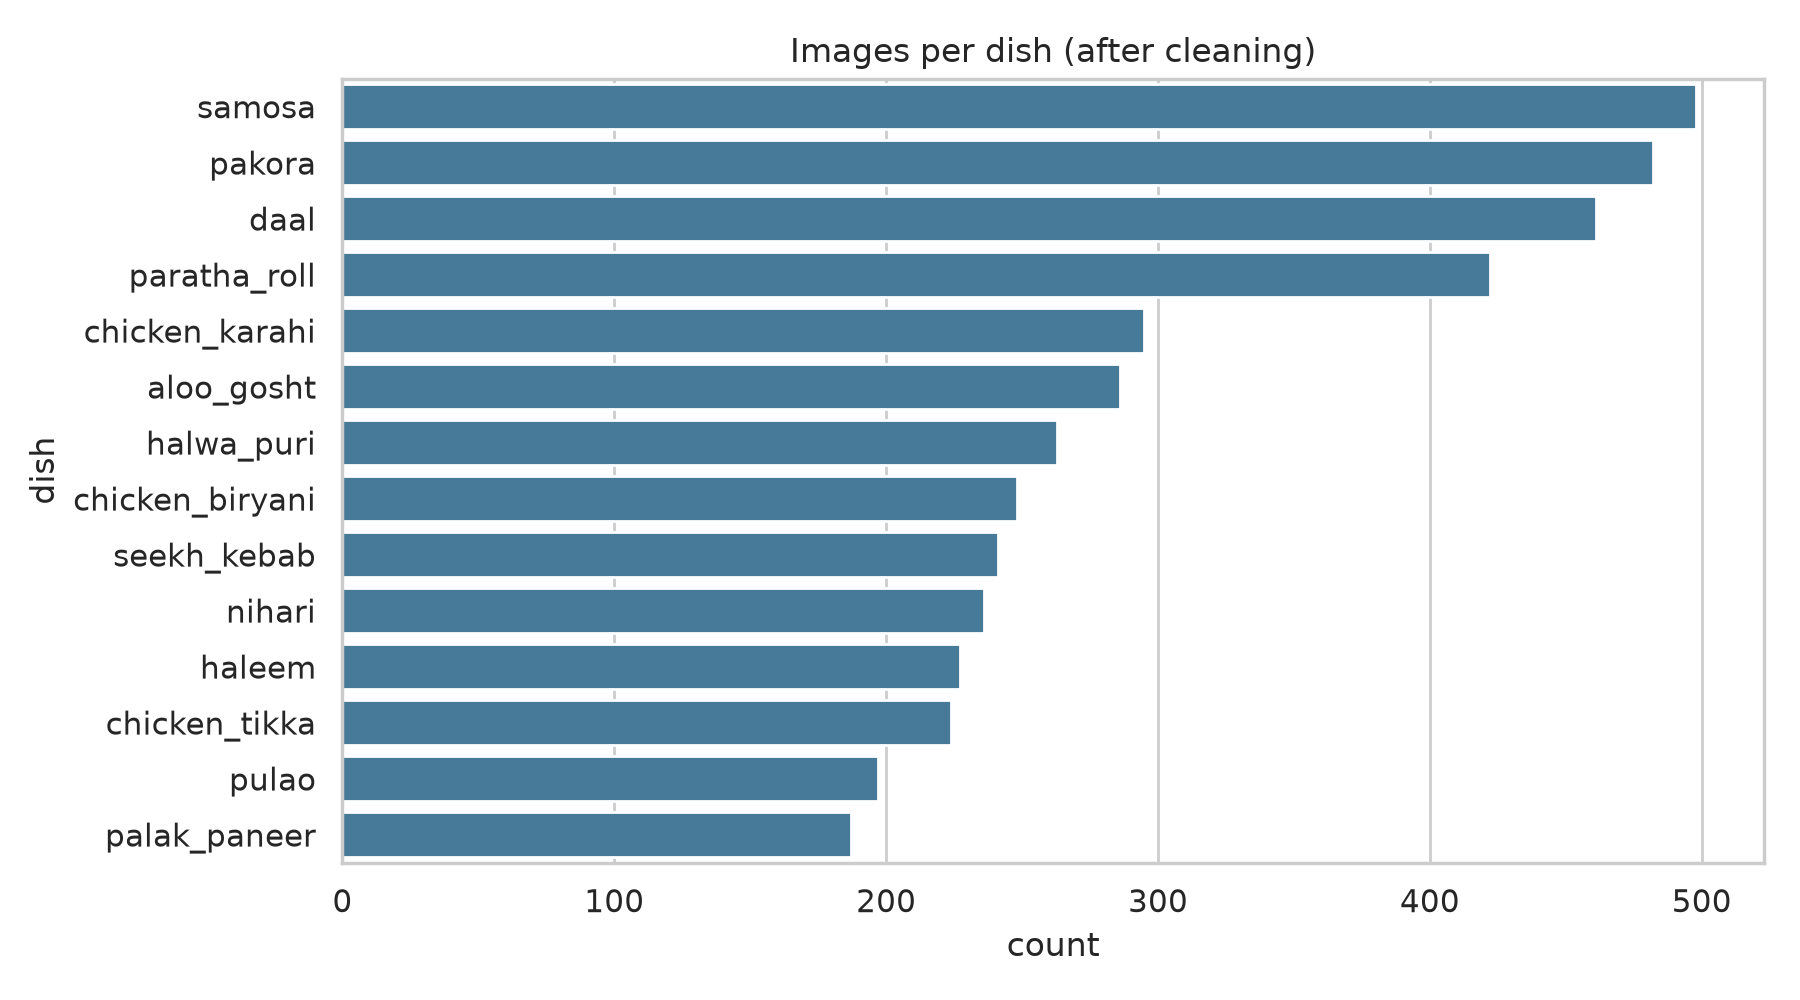
\includegraphics[width=0.85\textwidth]{class_distribution.png}
  \caption{Images per dish after cleaning.}
\end{figure}
The classes are imbalanced. Samosa has the most images (498) and palak\_paneer the fewest (187), a ratio of about 2.7 to 1. The four largest classes (samosa, pakora, daal and paratha\_roll) are the four dishes that also draw on the Kaggle dataset~\cite{jain_indian_food_kaggle}.

\begin{figure}[H]
  \centering
  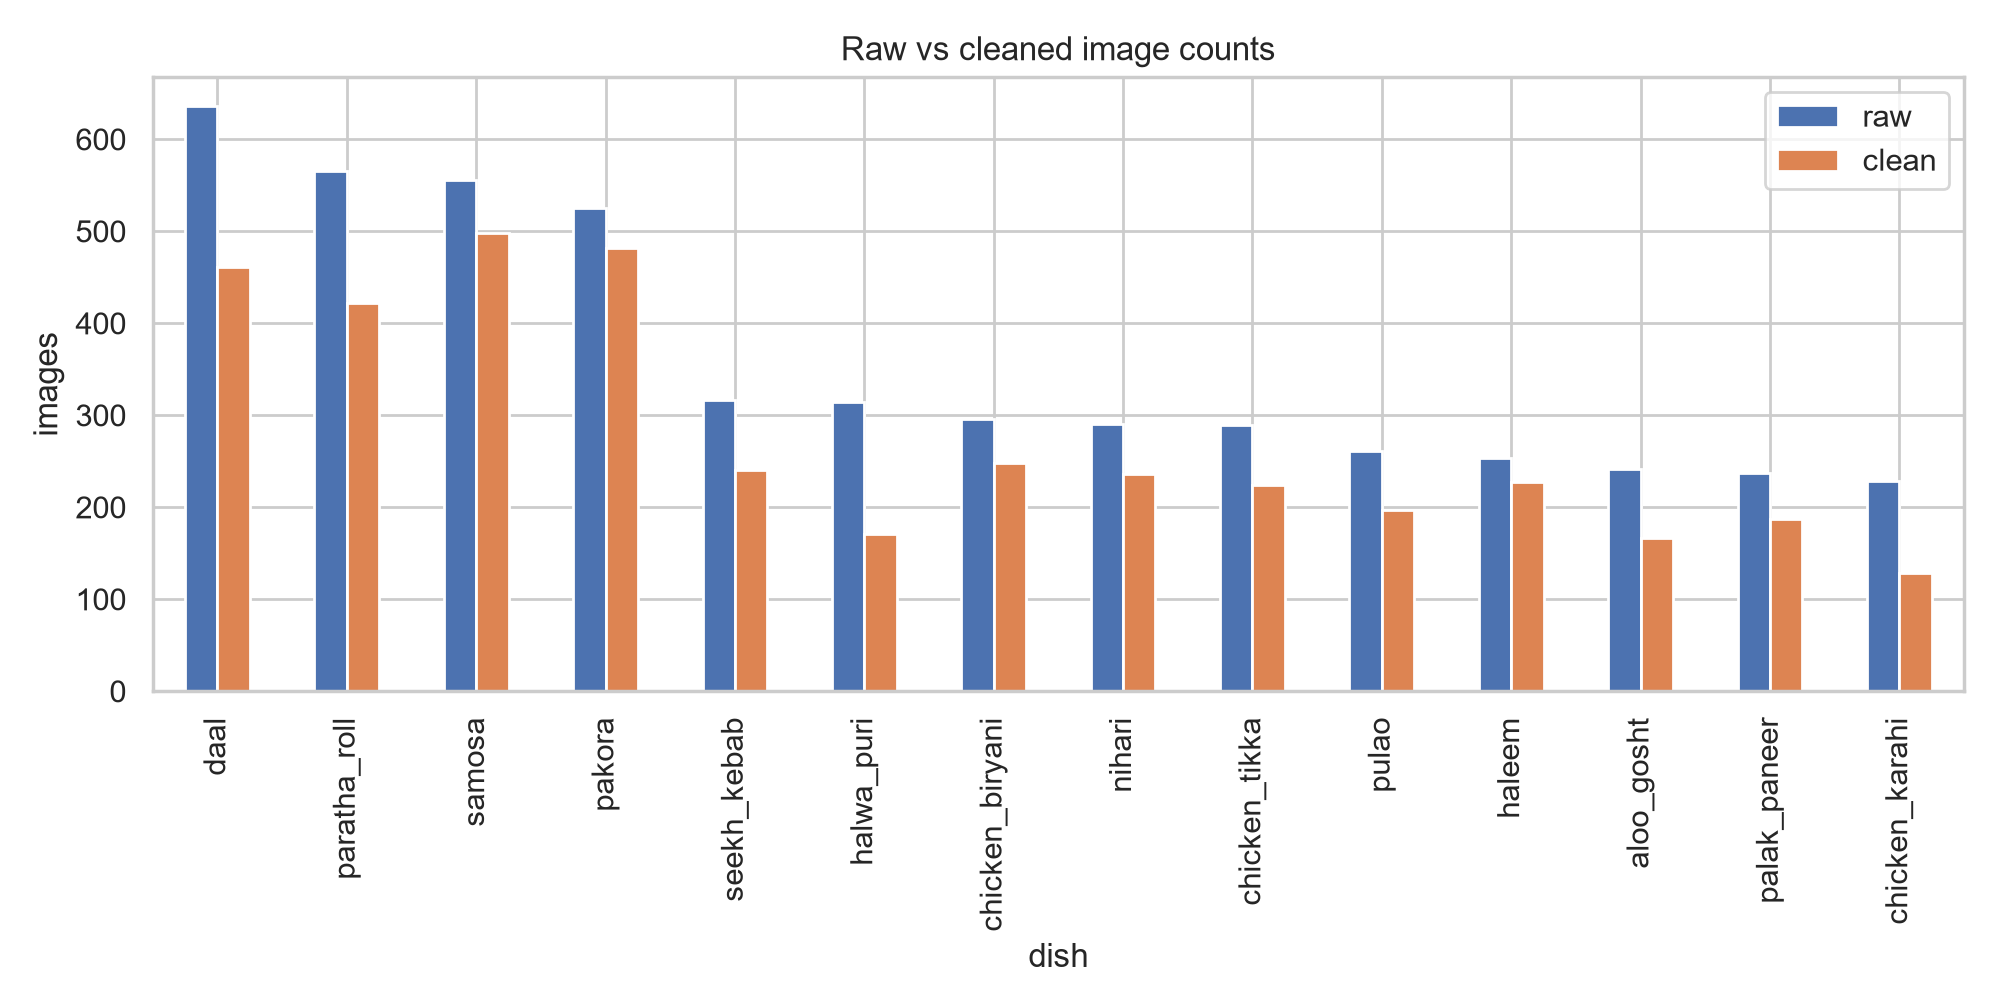
\includegraphics[width=0.85\textwidth]{raw_vs_clean.png}
  \caption{Raw versus cleaned image counts.}
\end{figure}
Cleaning reduced the collection from 6,193 to 4,267 images, and every dish lost some images. The largest shares were lost by halwa\_puri (439 of 702, about 63\%), aloo\_gosht (338 of 624, about 54\%) and chicken\_karahi (344 of 639, about 54\%), which are the three dishes that received top-up scraping and therefore contained many repeated downloads. Pakora lost the smallest share (43 of 525, about 8\%).

\begin{figure}[H]
  \centering
  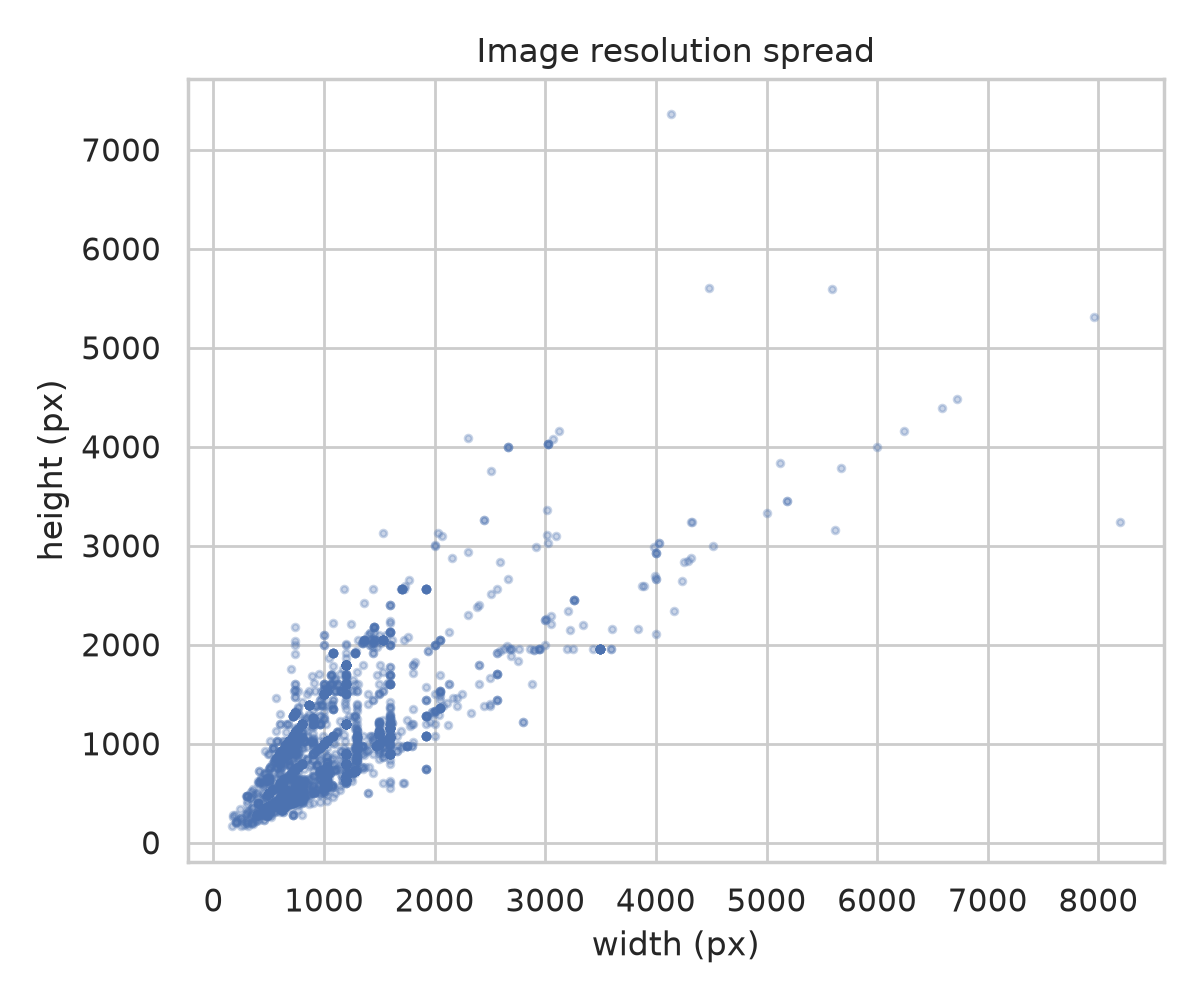
\includegraphics[width=0.6\textwidth]{image_sizes.png}
  \caption{Image resolution spread.}
\end{figure}
Image resolution varies widely, from small images of a few hundred pixels to a few very large ones more than 4,000 pixels wide, and width and height grow together. This spread motivates resizing everything to a common $224 \times 224$ input.

\begin{figure}[H]
  \centering
  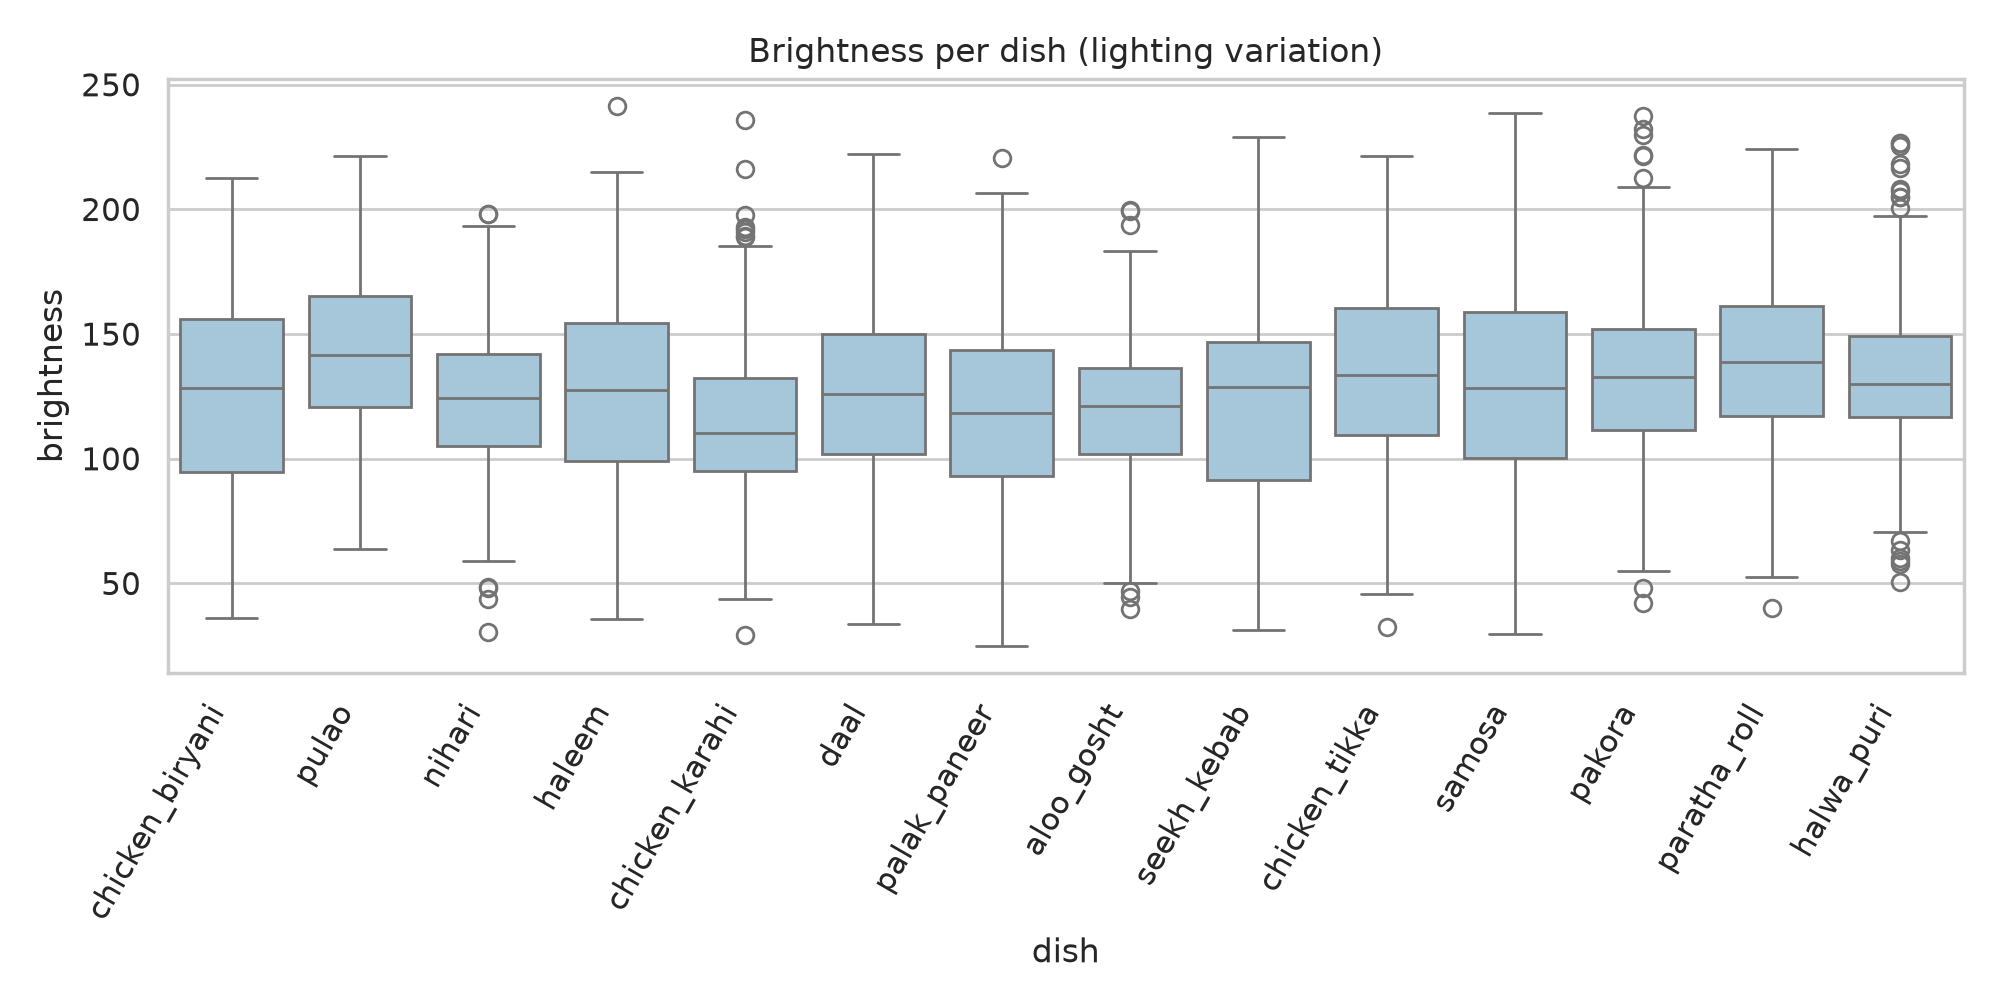
\includegraphics[width=0.85\textwidth]{brightness_per_dish.png}
  \caption{Brightness per dish (lighting variation).}
\end{figure}
Brightness varies widely within every dish, so each dish contains both dark and bright photos, and lighting differs between individual images more than it differs between dishes.

\begin{figure}[H]
  \centering
  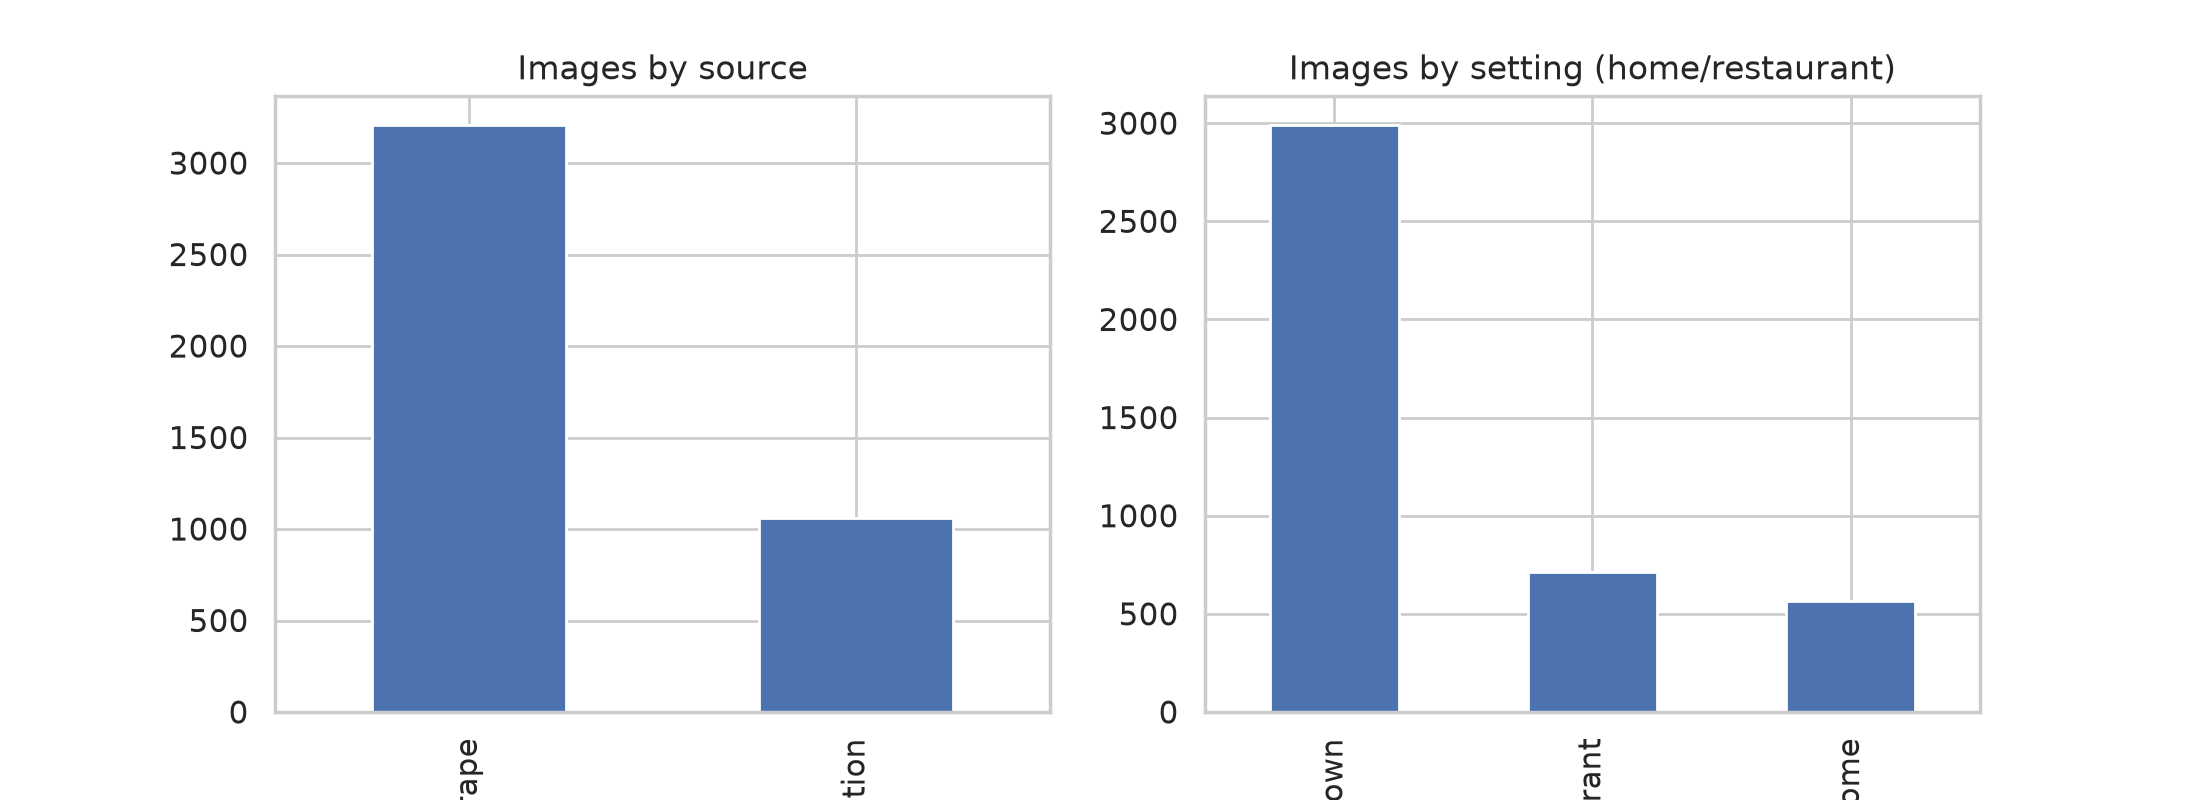
\includegraphics[width=0.85\textwidth]{source_and_setting.png}
  \caption{Images by source and by setting (home/restaurant).}
\end{figure}
Most of the cleaned images come from Bing, and a smaller share from the Kaggle dataset. The setting is unknown for most images, because only some of the search queries mention a home or restaurant setting and the Kaggle images carry no setting label.

\begin{figure}[H]
  \centering
  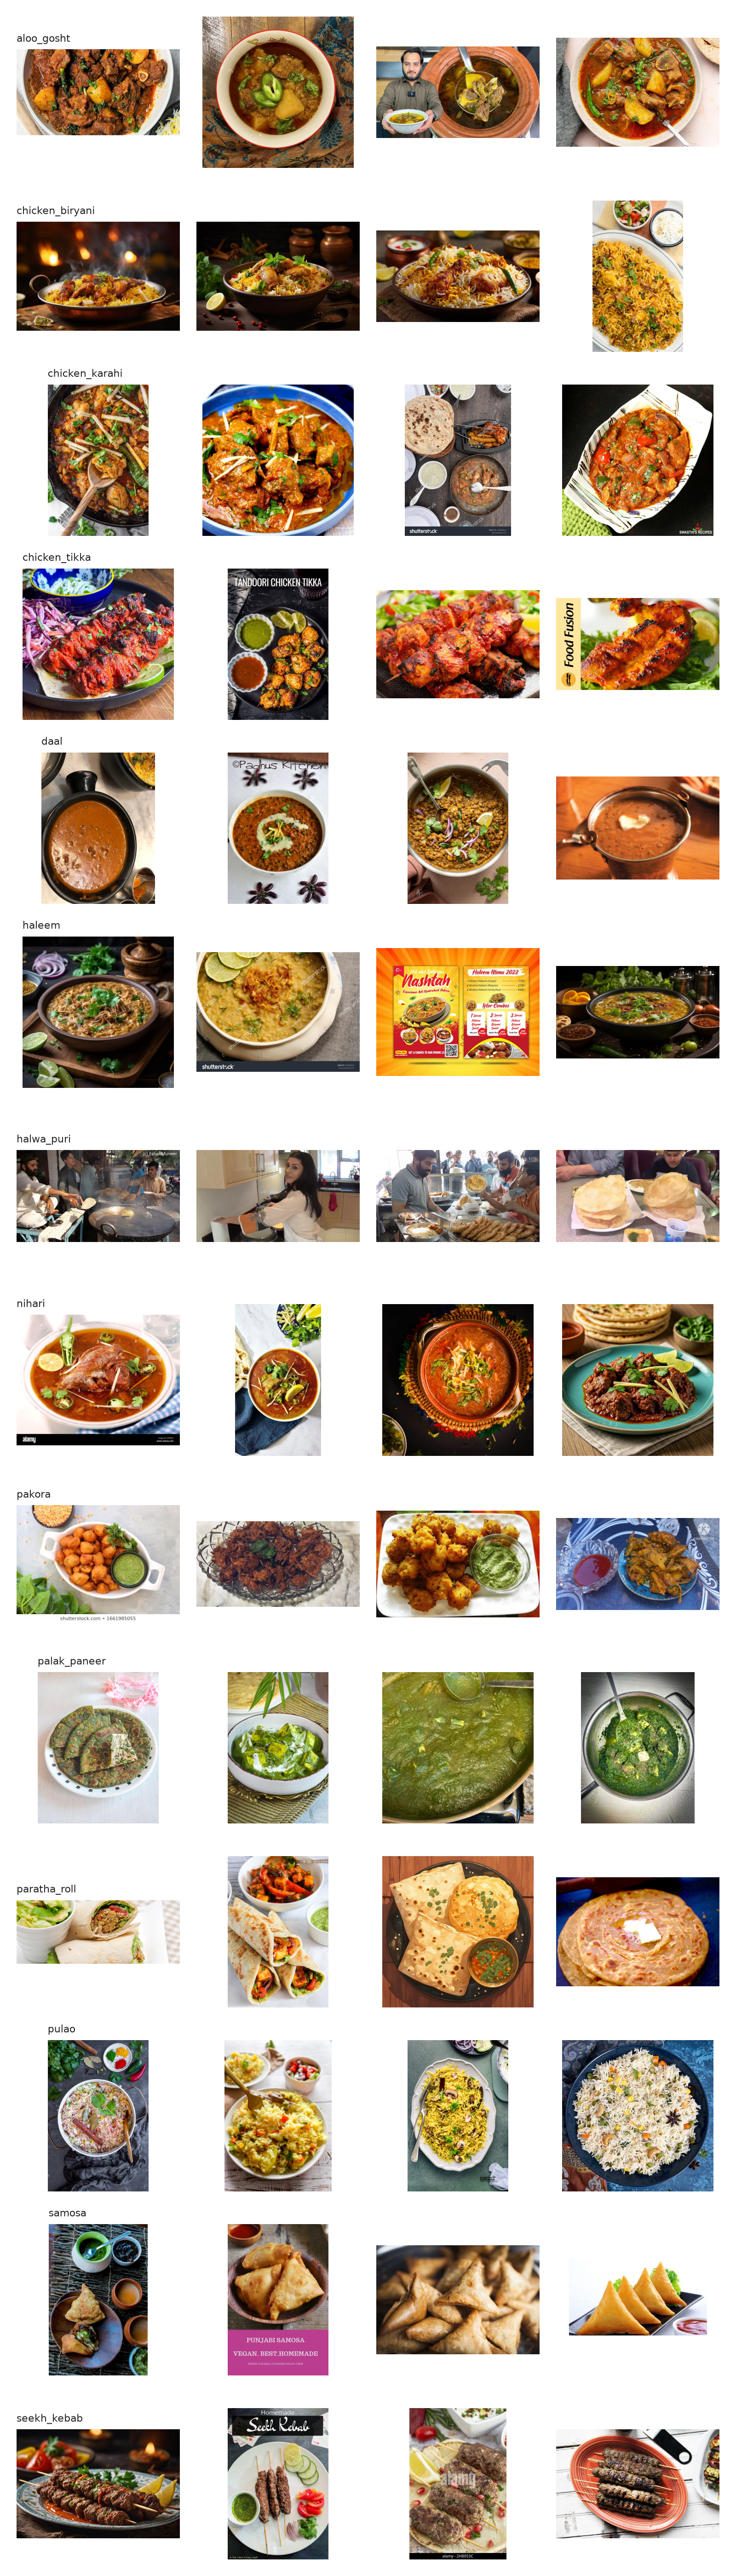
\includegraphics[width=0.7\textwidth,height=0.8\textheight,keepaspectratio]{sample_grid.png}
  \caption{Random samples per dish.}
\end{figure}
The sample grid shows four random cleaned images per dish. The images vary widely in angle, plating and background. The grid also exposes the problems listed under the data limitations, such as watermarks, text overlays and occasional images that do not show the labelled dish.

\subsection{Data Limitations}
\begin{itemize}
  \item \textbf{Watermarks and text overlays:} images scraped from Bing can contain watermarks, captions or text overlays, which the automatic blur and duplicate filters do not remove. Stock-photo watermarks (for example Alamy and Shutterstock), text banners (many in Urdu), video-thumbnail graphics with a ``subscribe'' button or a presenter's face, and even a menu page were found in the cleaned images. In a random sample of 24 images per dish, about half of the aloo\_gosht and halwa\_puri images (the dishes with the most top-up images) and about one in five chicken\_karahi images were affected. Some banners even repeat the dish name, so a model could learn to read the text instead of recognising the food.
  \item \textbf{Label noise:} a few cleaned images do not appear to show the labelled dish or are not photographs of food (for example a cartoon illustration and a plate of chaat among the halwa\_puri images, a restaurant menu page among the chicken\_karahi images, and off-topic images in palak\_paneer). The cleaning filters cannot detect these and the dataset was reviewed only by sampling, so some mislabelled images probably remain.
  \item \textbf{Source bias:} four dishes (samosa, pakora, daal and paratha\_roll) draw on a single Kaggle dataset, while the other ten come only from Bing. The two sources may differ in photographic style, so a model could partly learn the source instead of the dish.
  \item \textbf{Close substitutes:} the Kaggle classes \texttt{dal\_makhani} and \texttt{kaathi\_rolls} stand in for daal and paratha\_roll. They are similar dishes but not identical to what the project is meant to recognise.
  \item \textbf{Class imbalance:} raw counts range from 237 to 702 images per dish and cleaned counts from 187 to 498. All 14 dishes are above our 150-image target, but only after the top-up scraping (chicken\_karahi was at 128 after the first cleaning). The smallest class, palak\_paneer, has 187 images, so with a 15\% split its validation and test sets hold only about 28 images each and its per-class results will be noisy.
  \item \textbf{Repeated downloads:} the top-up queries returned many images that were already collected, so a large part of the new downloads was removed as duplicates. The three top-up dishes therefore keep a smaller share of their raw images than the others. Some near-duplicates still survive: in the aloo\_gosht sample, what appears to be the same photo occurs twice with different crops, which the perceptual-hash threshold did not catch.
  \item \textbf{Licensing:} the scraped images belong to their original owners. They were collected for academic use only and are not redistributed: the dataset is excluded from the repository.
\end{itemize}

\section{Models}

\subsection{Framework}
We implemented both models in \textbf{PyTorch}~\cite{paszke2019pytorch} with
\textbf{torchvision}. PyTorch provides a clean imperative interface for custom
training loops (frozen then unfrozen stages, early stopping, cosine schedules)
and torchvision ships EfficientNet-B0~\cite{tan2019efficientnet} with
ImageNet~\cite{deng2009imagenet} weights. The same scripts run on a Colab T4
GPU and on CPU. Scikit-learn~\cite{pedregosa2011sklearn} is used in
\texttt{src/evaluate.py} for computing evaluation metrics.

\subsection{EfficientNet-B0 (transfer learning)}
The main model is torchvision EfficientNet-B0~\cite{tan2019efficientnet}
pretrained on ImageNet~\cite{deng2009imagenet} (\texttt{IMAGENET1K\_V1}). The
original classifier is replaced by Dropout then a linear layer to 14 logits.
Input tensors are $3 \times 224 \times 224$, matching the resized JPEGs from
Section~2. After the backbone, EfficientNet applies global average pooling to a
1280-dimensional vector, then our classification head.

Training has two stages, implemented in \texttt{src/train.py}:
\begin{enumerate}
  \item \textbf{Head (5 epochs).} The backbone is frozen. Only Dropout and
        the linear layer are trained, at learning rate $1 \times 10^{-3}$.
  \item \textbf{Fine-tune.} The last 3 entries of \texttt{model.features}
        are unfrozen. Training continues at $1 \times 10^{-4}$ with a fresh
        AdamW~\cite{loshchilov2019adamw} optimiser and cosine scheduler,
        starting from the best head checkpoint.
\end{enumerate}
Two stages keep the pretrained filters from being destroyed in the first
epochs, then allow the last blocks to adapt to desi food photos.

\begin{figure}[H]
  \centering
  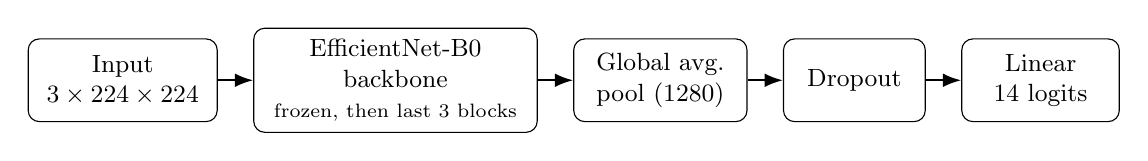
\begin{tikzpicture}[
      font=\small,
      box/.style={draw, rounded corners, align=center, minimum height=1.05cm, inner sep=4pt},
      arr/.style={-{Latex}, thick}
    ]
    \node[box, minimum width=2.4cm] (in) {Input\\$3 \times 224 \times 224$};
    \node[box, minimum width=3.6cm, right=0.45cm of in] (bb) {EfficientNet-B0\\backbone\\{\scriptsize frozen, then last 3 blocks}};
    \node[box, minimum width=2.2cm, right=0.45cm of bb] (gap) {Global avg.\\pool (1280)};
    \node[box, minimum width=1.8cm, right=0.45cm of gap] (drop) {Dropout};
    \node[box, minimum width=2.0cm, right=0.45cm of drop] (fc) {Linear\\14 logits};
    \draw[arr] (in) -- (bb);
    \draw[arr] (bb) -- (gap);
    \draw[arr] (gap) -- (drop);
    \draw[arr] (drop) -- (fc);
  \end{tikzpicture}
  \caption{EfficientNet-B0 transfer pipeline used in \texttt{src/efficientnet\_model.py}.}
\end{figure}

\subsection{Baseline CNN}
\texttt{src/baseline\_cnn.py} implements our from-scratch comparison network.
The shared contract uses the same input and output interface as EfficientNet:
class \texttt{BaselineCNN(num\_classes=14)}, input $3 \times 224 \times 224$,
output 14 logits, trained with \texttt{python src/train.py --model baseline}.
Its full layer table, block diagram, and fixed hyperparameters are detailed in
Section~4.

\subsection{Loss, optimiser, schedule, regularisation}
\begin{itemize}
  \item \textbf{Loss.} Cross-entropy with label smoothing $0.1$. Smoothing
        stops the head from becoming over-confident on noisy Bing labels
        (Section~2 noted watermarks and a little label noise).
  \item \textbf{Optimiser.} AdamW~\cite{loshchilov2019adamw} on \emph{trainable}
        parameters only, with weight decay $1 \times 10^{-4}$. AdamW is a
        standard default for CNN fine-tuning; excluding frozen weights avoids
        useless states in the optimiser.
  \item \textbf{Scheduler.} Cosine annealing over the epochs of each stage.
        The learning rate falls smoothly and does not need an extra validation
        rule (unlike ReduceLROnPlateau).
  \item \textbf{Early stopping.} Training watches validation loss with
        patience 5 and writes the best weights under \texttt{checkpoints/}
        as \texttt{efficientnet\_best.pt}.
  \item \textbf{Augmentation (train only).} RandomResizedCrop 224 (scale
        $0.8$--$1.0$), horizontal flip, rotation of about $15^{\circ}$, and
        ColorJitter (brightness and contrast $0.2$). Validation and test
        only resize to $224 \times 224$.
  \item \textbf{Normalisation.} ImageNet mean $(0.485, 0.456, 0.406)$ and
        std $(0.229, 0.224, 0.225)$, as named constants in
        \texttt{src/dataset.py}. Although Section~2 recorded train-set
        statistics in \texttt{norm\_stats.json}, we use ImageNet normalisation
        because the EfficientNet weights were pretrained with those statistics;
        mixing the two scales would shift every activation in the frozen
        backbone.
\end{itemize}

\subsection{Hyperparameter search}
\texttt{src/tune.py} changes \emph{one} factor at a time around a default
(head lr $1 \times 10^{-3}$, fine-tune lr $1 \times 10^{-4}$, batch 32,
dropout $0.3$, weight decay $1 \times 10^{-4}$, label smoothing $0.1$).
Each trial ran at most 8 epochs on a Colab T4, without writing a test-pred
file. Table~\ref{tab:hparam} is copied from \texttt{results/hparam\_results.csv}.
The best row (lowest validation loss) is in bold.

\begin{table}[H]
  \centering
  \small
  \begin{tabular}{|l|r|r|r|r|r|}
    \hline
    \textbf{Run} & \textbf{lr} & \textbf{Batch} & \textbf{Drop.} & \textbf{Val.\ loss} & \textbf{Val.\ acc.} \\
    \hline
    default      & 0.001  & 32 & 0.3 & 1.190 & 0.777 \\
    lr\_3e-4     & 0.0003 & 32 & 0.3 & 1.194 & 0.773 \\
    lr\_1e-4     & 0.0001 & 32 & 0.3 & 1.238 & 0.767 \\
    \textbf{batch\_16} & \textbf{0.001} & \textbf{16} & \textbf{0.3} & \textbf{1.167} & \textbf{0.792} \\
    batch\_64    & 0.001  & 64 & 0.3 & 1.217 & 0.769 \\
    dropout\_0.2 & 0.001  & 32 & 0.2 & 1.187 & 0.781 \\
    dropout\_0.5 & 0.001  & 32 & 0.5 & 1.200 & 0.775 \\
    wd\_1e-2     & 0.001  & 32 & 0.3 & 1.190 & 0.777 \\
    \hline
  \end{tabular}
  \caption{One-factor EfficientNet search (\texttt{results/hparam\_results.csv}).
  Fine-tune lr $1 \times 10^{-4}$, weight decay $1 \times 10^{-4}$ except
  \texttt{wd\_1e-2} ($1 \times 10^{-2}$), label smoothing $0.1$ throughout.
  Accuracies are the CSV \texttt{best\_val\_acc} values.}
  \label{tab:hparam}
\end{table}

Lowering the head learning rate or raising the batch size made validation
loss worse than the default. Dropout $0.2$ was slightly better than $0.3$ on
accuracy ($0.781$ vs $0.777$) and loss ($1.187$ vs $1.190$). Weight decay
$1 \times 10^{-2}$ matched the default loss ($1.190$). \textbf{Batch size 16}
clearly reduced validation loss ($1.167$ vs $1.190$) and raised validation
accuracy to $0.792$, so the final EfficientNet run used batch size 16 and
otherwise the default settings: 20 epochs, 5 head epochs, last 3 blocks
unfrozen, dropout $0.3$, AdamW weight decay $1 \times 10^{-4}$, and label
smoothing $0.1$.

From \texttt{results/history\_efficientnet.csv}, that full 20-epoch run reached
its best validation loss at epoch 19 (validation loss $1.0688$, validation
accuracy $0.8297$) during fine-tuning. Section~4 presents the training curves
and held-out test metrics for both models.

\section{Training and Evaluation}

\subsection{Baseline CNN design}
The baseline is a small convolutional network trained from scratch
(\texttt{src/baseline\_cnn.py}, class \texttt{BaselineCNN}). It is the
reference point for the pretrained EfficientNet-B0~\cite{tan2019efficientnet}. It takes a
$3 \times 224 \times 224$ image and returns 14 logits (no softmax inside the
model). It has four convolution blocks, each made of a $3 \times 3$
convolution (padding 1), batch normalisation, ReLU and $2 \times 2$ max
pooling, with 32, 64, 128 and 256 channels. Global average pooling,
dropout ($0.3$) and one linear layer follow. The model has
\textbf{392,974} trainable parameters.

\begin{table}[H]
  \centering
  \begin{tabular}{|l|l|r|}
    \hline
    \textbf{Layer} & \textbf{Output size} & \textbf{Parameters} \\ \hline
    Input & $3 \times 224 \times 224$ & 0 \\ \hline
    Conv 3$\to$32 + BatchNorm + ReLU & $32 \times 224 \times 224$ & 960 \\ \hline
    MaxPool 2 & $32 \times 112 \times 112$ & 0 \\ \hline
    Conv 32$\to$64 + BatchNorm + ReLU & $64 \times 112 \times 112$ & 18,624 \\ \hline
    MaxPool 2 & $64 \times 56 \times 56$ & 0 \\ \hline
    Conv 64$\to$128 + BatchNorm + ReLU & $128 \times 56 \times 56$ & 74,112 \\ \hline
    MaxPool 2 & $128 \times 28 \times 28$ & 0 \\ \hline
    Conv 128$\to$256 + BatchNorm + ReLU & $256 \times 28 \times 28$ & 295,680 \\ \hline
    MaxPool 2 & $256 \times 14 \times 14$ & 0 \\ \hline
    Global average pooling & $256$ & 0 \\ \hline
    Dropout (0.3) & $256$ & 0 \\ \hline
    Linear 256$\to$14 & $14$ logits & 3,598 \\ \hline
    \textbf{Total} & & \textbf{392,974} \\ \hline
  \end{tabular}
  \caption{Baseline CNN layers. Parameter counts include the batch-norm
  weights and biases.}
\end{table}

\begin{figure}[H]
  \centering
  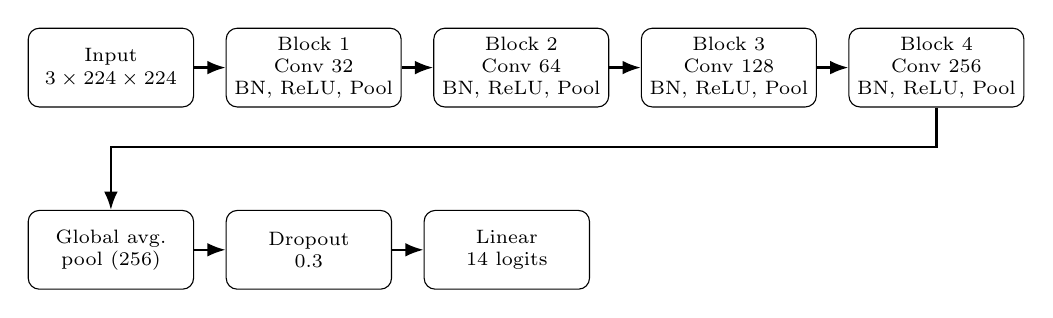
\begin{tikzpicture}[
      font=\scriptsize,
      box/.style={draw, rounded corners, align=center, minimum height=1.0cm, minimum width=2.1cm, inner sep=3pt},
      arr/.style={-{Latex}, thick}
    ]
    \node[box] (in) {Input\\$3 \times 224 \times 224$};
    \node[box, right=0.4cm of in] (b1) {Block 1\\Conv 32\\BN, ReLU, Pool};
    \node[box, right=0.4cm of b1] (b2) {Block 2\\Conv 64\\BN, ReLU, Pool};
    \node[box, right=0.4cm of b2] (b3) {Block 3\\Conv 128\\BN, ReLU, Pool};
    \node[box, right=0.4cm of b3] (b4) {Block 4\\Conv 256\\BN, ReLU, Pool};
    \node[box, below=1.3cm of in] (gap) {Global avg.\\pool (256)};
    \node[box, right=0.4cm of gap] (drop) {Dropout\\0.3};
    \node[box, right=0.4cm of drop] (fc) {Linear\\14 logits};
    \draw[arr] (in) -- (b1);
    \draw[arr] (b1) -- (b2);
    \draw[arr] (b2) -- (b3);
    \draw[arr] (b3) -- (b4);
    \draw[arr] (b4.south) -- ++(0,-0.5) -| (gap.north);
    \draw[arr] (gap) -- (drop);
    \draw[arr] (drop) -- (fc);
  \end{tikzpicture}
  \caption{Baseline CNN block diagram (\texttt{src/baseline\_cnn.py}).}
\end{figure}

The loss is cross-entropy with label smoothing $0.1$. The optimiser is
AdamW~\cite{loshchilov2019adamw} with a cosine-annealing learning-rate schedule.
These are the same settings as for EfficientNet, because both models use the
shared trainer \texttt{src/train.py}.

\subsection{Baseline hyperparameters}
The baseline was trained \textbf{once} with fixed values. It was not tuned.
The EfficientNet hyperparameter search is described in Section~3.

\begin{table}[H]
  \centering
  \begin{tabular}{|l|l|p{7.2cm}|}
    \hline
    \textbf{Hyperparameter} & \textbf{Value} & \textbf{Justification} \\ \hline
    Learning rate & $1 \times 10^{-3}$ & Usual AdamW starting value for training a small CNN from scratch. \\ \hline
    Batch size & 32 & Fits comfortably on a Colab T4 GPU and gives stable batch-norm statistics. \\ \hline
    Dropout & 0.3 & Moderate regularisation before the single linear layer. \\ \hline
    Weight decay & $1 \times 10^{-4}$ & Light L2-style regularisation; same value as the EfficientNet runs. \\ \hline
    Label smoothing & 0.1 & Reduces over-confidence on noisy scraped labels; same as EfficientNet. \\ \hline
    Epochs run & 20 (maximum 20) & Early stopping (patience 5) did not trigger; the cosine schedule was set for 20 epochs. \\ \hline
  \end{tabular}
  \caption{Baseline hyperparameters. Training command:
  \texttt{python src/train.py --model baseline --epochs 20 --batch-size 32
  --lr 1e-3 --weight-decay 1e-4 --label-smoothing 0.1 --num-workers 2}.}
\end{table}

\subsection{Validation strategy}
We use the 70/15/15 stratified train/validation/test split made in Section~2
(seed 42), which gives 2,986 training, 640 validation and 641 test images.
The validation set is used during training for early stopping and for
choosing the best checkpoint. The test set is used once, at the end, to
produce the predictions evaluated below. We did not use K-fold
cross-validation: the held-out test set is fixed from Section~2, and
repeated training of the EfficientNet model would be costly.

\subsection{Training curves}
Figure~\ref{fig:curves-baseline} shows the baseline's loss and accuracy per
epoch. Over the 20 epochs the validation loss fell to $1.7605$ and
validation accuracy rose to $0.5422$, while training accuracy reached
$0.5271$ at epoch 20 and peaked at $0.5285$ at epoch 19
(\texttt{results/history\_baseline.csv}). Both curves were still
improving at epoch 20, so the baseline is probably under-trained; with
fixed settings and a single run we did not train it for longer. Training
accuracy stays close to validation accuracy, so there is no strong sign
of over-fitting.

\begin{figure}[H]
  \centering
  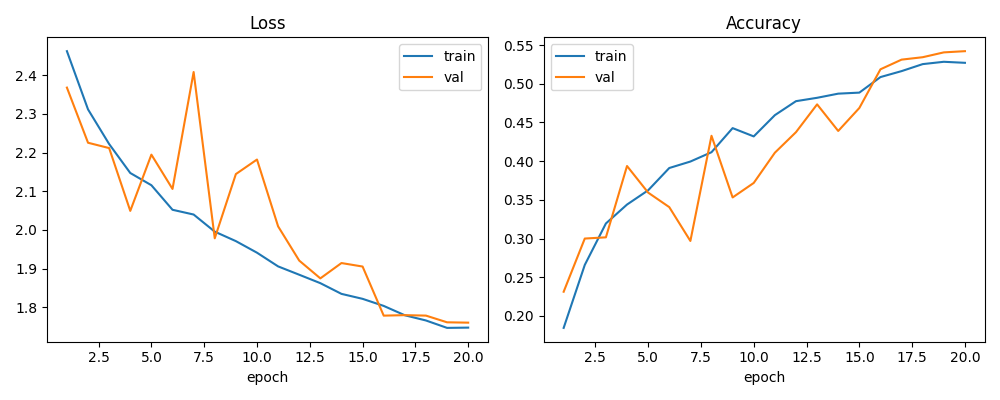
\includegraphics[width=0.9\textwidth]{curves_baseline.png}
  \caption{Baseline CNN training and validation curves.}
  \label{fig:curves-baseline}
\end{figure}

Figure~\ref{fig:curves-efficientnet} shows the EfficientNet-B0 curves
(final 20-epoch run, batch size 16). The dashed vertical line marks epoch 6,
where the last three backbone blocks are unfrozen for fine-tuning. Both curves
improve sharply after unfreezing. Best validation loss is reached at epoch 19
(validation loss $1.0688$, validation accuracy $0.8297$, training accuracy
$0.9401$), and in epoch 20 the model reaches a training accuracy of $0.9411$
and a validation accuracy of $0.8219$ with a validation loss of $1.0809$
(\texttt{results/history\_efficientnet.csv}). The gap of about 11 to 12
percentage points between training and validation accuracy points to moderate
over-fitting, whereas the baseline's two accuracies stayed close together. The
losses stay well above zero partly because of label smoothing ($0.1$).

\begin{figure}[H]
  \centering
  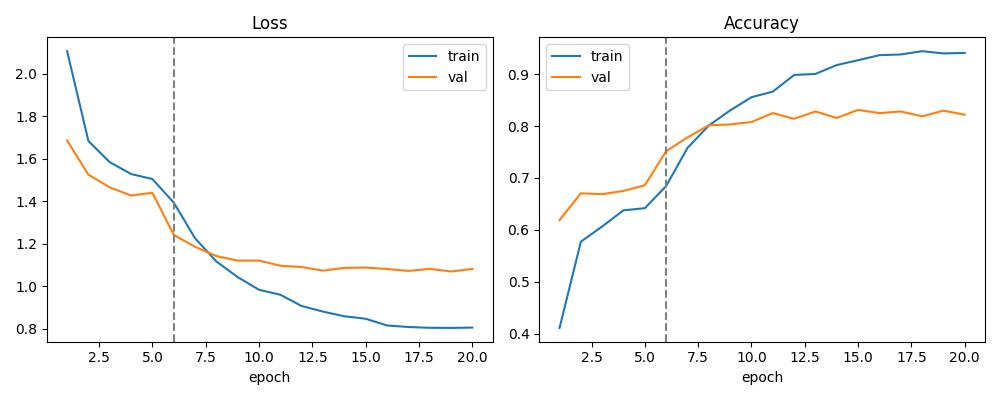
\includegraphics[width=0.9\textwidth]{curves_efficientnet.png}
  \caption{EfficientNet-B0 training and validation curves.}
  \label{fig:curves-efficientnet}
\end{figure}
\subsection{Evaluation metrics and why they fit}
The 14 classes are imbalanced (Section~2): \texttt{palak\_paneer} has 187
images and \texttt{samosa} 498. Accuracy alone can hide weak classes, so we
also report (computed with scikit-learn~\cite{pedregosa2011sklearn}):
\begin{itemize}
  \item \textbf{Precision and recall per dish}: precision says how often a
        predicted dish is right, recall says how many true images of a dish
        were found. Together they show each dish's errors.
  \item \textbf{Macro F1}: the mean F1 over the 14 dishes, so every dish has
        equal weight regardless of size.
  \item \textbf{AUC-ROC (one-vs-rest)}: uses the predicted probabilities,
        not only the top choice, so it shows how well a model ranks the
        correct dish.
  \item \textbf{Confusion matrix}: shows which dishes are mixed up.
\end{itemize}
All metrics are computed on the 641 test images by \texttt{src/evaluate.py}
from the prediction files \texttt{results/preds\_baseline\_test.csv} and
\texttt{results/preds\_efficientnet\_test.csv}.

\subsection{Results}
\begin{table}[H]
  \centering
  \begin{tabular}{|l|r|r|}
    \hline
    \textbf{Metric} & \textbf{Baseline CNN} & \textbf{EfficientNet-B0} \\ \hline
    Accuracy        & 0.5086 & 0.7988 \\ \hline
    Macro precision & 0.5044 & 0.7830 \\ \hline
    Macro recall    & 0.4799 & 0.7778 \\ \hline
    Macro F1        & 0.4700 & 0.7785 \\ \hline
    Macro AUC-ROC   & 0.8915 & 0.9706 \\ \hline
  \end{tabular}
  \caption{Test-set results (641 images), from
  \texttt{results/metrics\_baseline.csv} and
  \texttt{results/metrics\_efficientnet.csv}.}
\end{table}

\begin{table}[H]
  \centering
  \begin{tabular}{|l|r|r|r|}
    \hline
    \textbf{Dish} & \textbf{Test images} & \textbf{Baseline F1} & \textbf{EfficientNet F1} \\ \hline
    aloo\_gosht      & 43 & 0.364 & 0.783 \\ \hline
    chicken\_biryani & 37 & 0.473 & 0.649 \\ \hline
    chicken\_karahi  & 45 & 0.400 & 0.703 \\ \hline
    chicken\_tikka   & 33 & 0.233 & 0.698 \\ \hline
    daal             & 69 & 0.521 & 0.849 \\ \hline
    haleem           & 34 & 0.174 & 0.706 \\ \hline
    halwa\_puri      & 40 & 0.623 & 0.811 \\ \hline
    nihari           & 35 & 0.410 & 0.757 \\ \hline
    pakora           & 73 & 0.545 & 0.808 \\ \hline
    palak\_paneer    & 28 & 0.800 & 0.867 \\ \hline
    paratha\_roll    & 64 & 0.600 & 0.873 \\ \hline
    pulao            & 29 & 0.360 & 0.604 \\ \hline
    samosa           & 75 & 0.719 & 0.940 \\ \hline
    seekh\_kebab     & 36 & 0.357 & 0.853 \\ \hline
  \end{tabular}
  \caption{Per-dish F1 on the test set.}
  \label{tab:f1}
\end{table}

EfficientNet-B0 has a higher F1 than the baseline for every dish. The
largest gains are for \texttt{haleem} (0.174 to 0.706), \texttt{seekh\_kebab}
(0.357 to 0.853) and \texttt{chicken\_tikka} (0.233 to 0.698).

\begin{figure}[H]
  \centering
  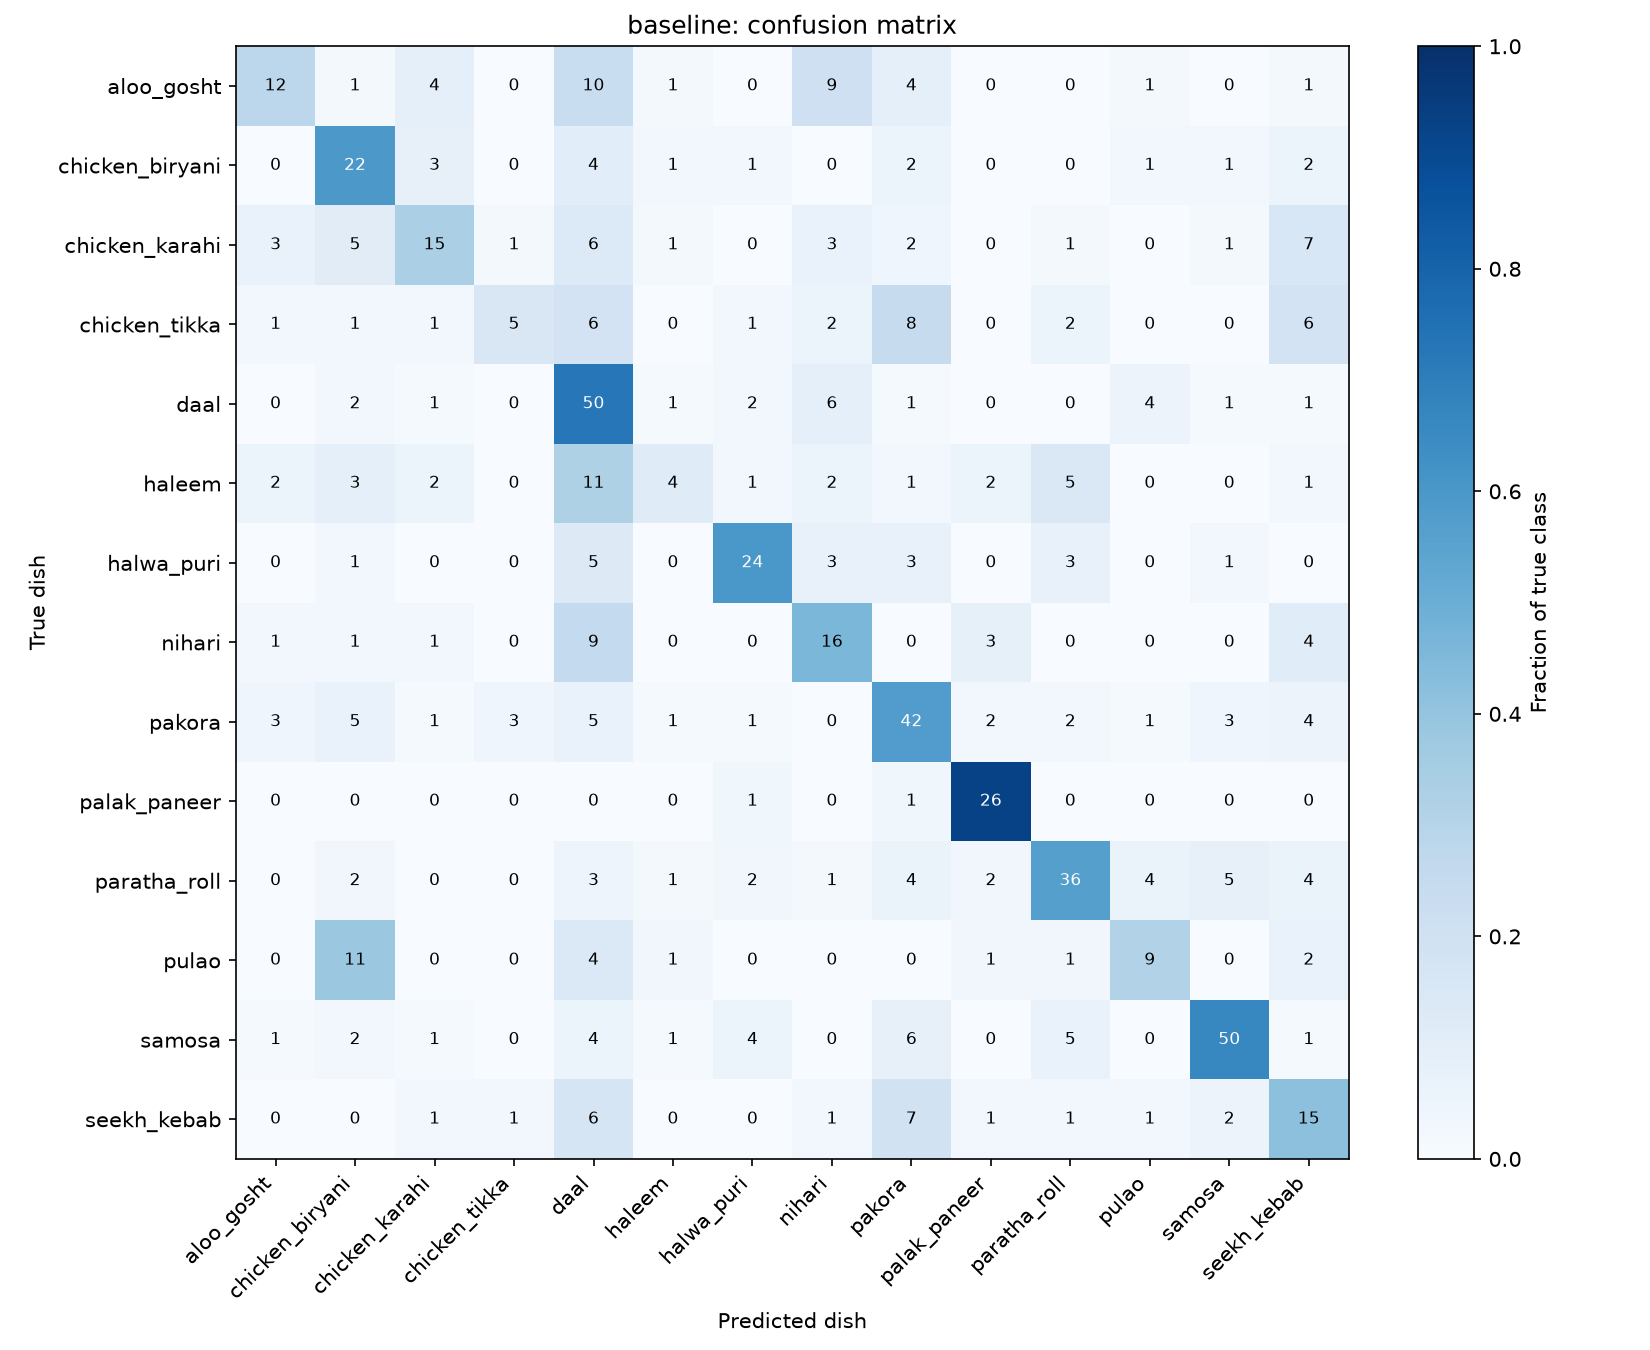
\includegraphics[width=0.85\textwidth]{confusion_baseline.png}
  \caption{Baseline CNN confusion matrix (row-normalised, counts in cells).}
\end{figure}

\begin{figure}[H]
  \centering
  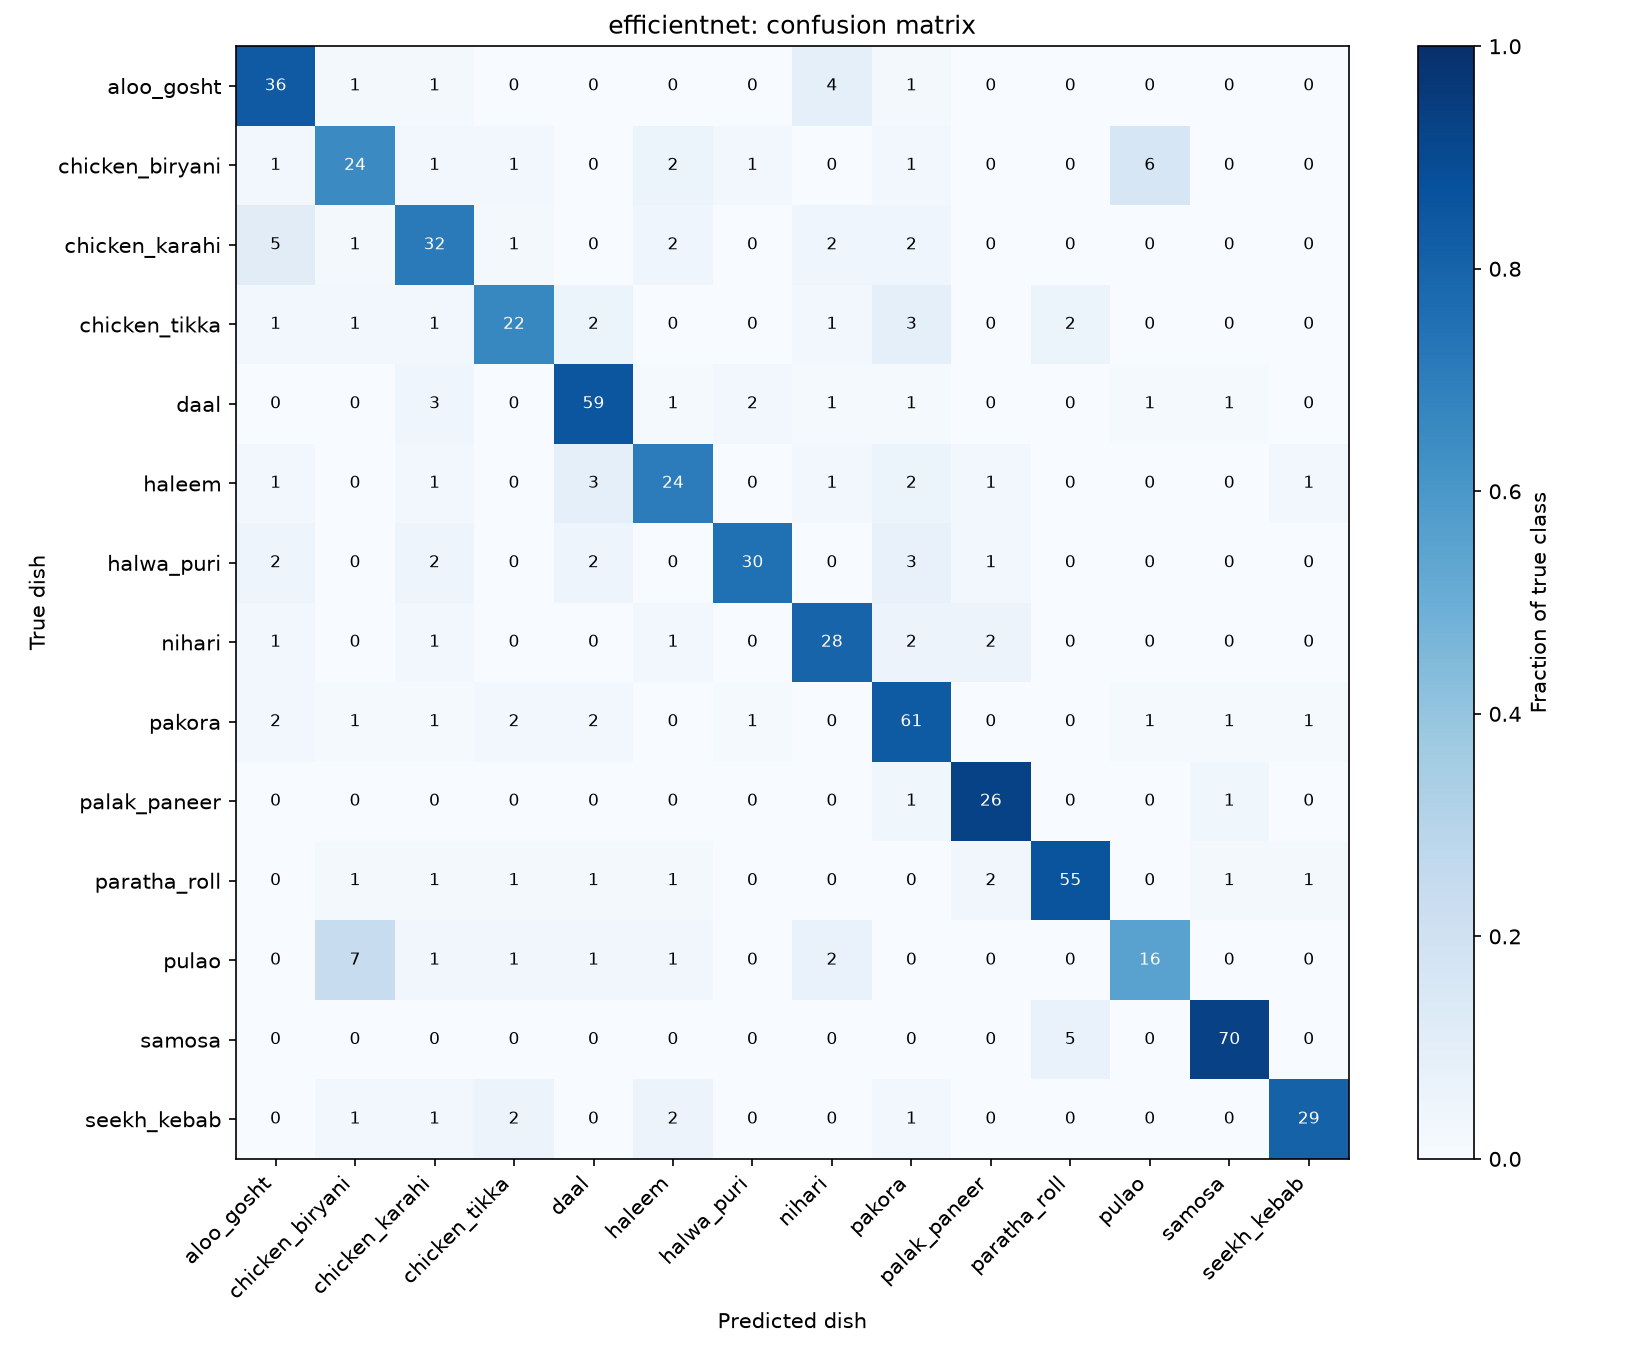
\includegraphics[width=0.85\textwidth]{confusion_efficientnet.png}
  \caption{EfficientNet-B0 confusion matrix (row-normalised, counts in cells).}
\end{figure}
\subsection{Error analysis}
\textbf{Weakest dishes.} Table~\ref{tab:worst} lists the three dishes with
the lowest recall (accuracy within the dish) for each model, from
\texttt{results/\allowbreak bias\_\allowbreak baseline\_\allowbreak class.csv} and
\texttt{results/\allowbreak bias\_\allowbreak efficientnet\_\allowbreak class.csv}.

\begin{table}[H]
  \centering
  \begin{tabular}{|l|l|r|r|}
    \hline
    \textbf{Model} & \textbf{Dish} & \textbf{Test images} & \textbf{Recall} \\ \hline
    Baseline     & haleem           & 34 & 0.118 \\ \hline
    Baseline     & chicken\_tikka   & 33 & 0.152 \\ \hline
    Baseline     & aloo\_gosht      & 43 & 0.279 \\ \hline
    EfficientNet & pulao            & 29 & 0.552 \\ \hline
    EfficientNet & chicken\_biryani & 37 & 0.649 \\ \hline
    EfficientNet & chicken\_tikka   & 33 & 0.667 \\ \hline
  \end{tabular}
  \caption{Three weakest dishes per model by recall.}
  \label{tab:worst}
\end{table}

{\sloppy
\textbf{Confused pairs.} For EfficientNet the most frequent errors
(\texttt{bias\_\allowbreak efficientnet\_\allowbreak confusions.csv}) are \texttt{pulao}
predicted as \texttt{chicken\_biryani} (7 images) and
\texttt{chicken\_biryani} predicted as \texttt{pulao} (6), followed by
\texttt{chicken\_karahi} as \texttt{aloo\_gosht} (5) and \texttt{samosa} as
\texttt{paratha\_roll} (5). These look-alike dishes are plausibly confused
because of similar appearance, though we did not test this. The baseline's
top errors (\texttt{results/\allowbreak bias\_\allowbreak baseline\_\allowbreak confusions.csv}) are
\texttt{haleem} as \texttt{daal} (11), \texttt{pulao} as
\texttt{chicken\_biryani} (11), \texttt{aloo\_gosht} as \texttt{daal} (10)
and \texttt{aloo\_gosht} as \texttt{nihari} (9). Many of its errors involve
stew-like dishes such as haleem, nihari, aloo\_gosht and daal.
\par}

\textbf{Failure examples.} Figure~\ref{fig:failures} shows misclassified test
images from EfficientNet (random sample, seed 42).

\begin{figure}[H]
  \centering
  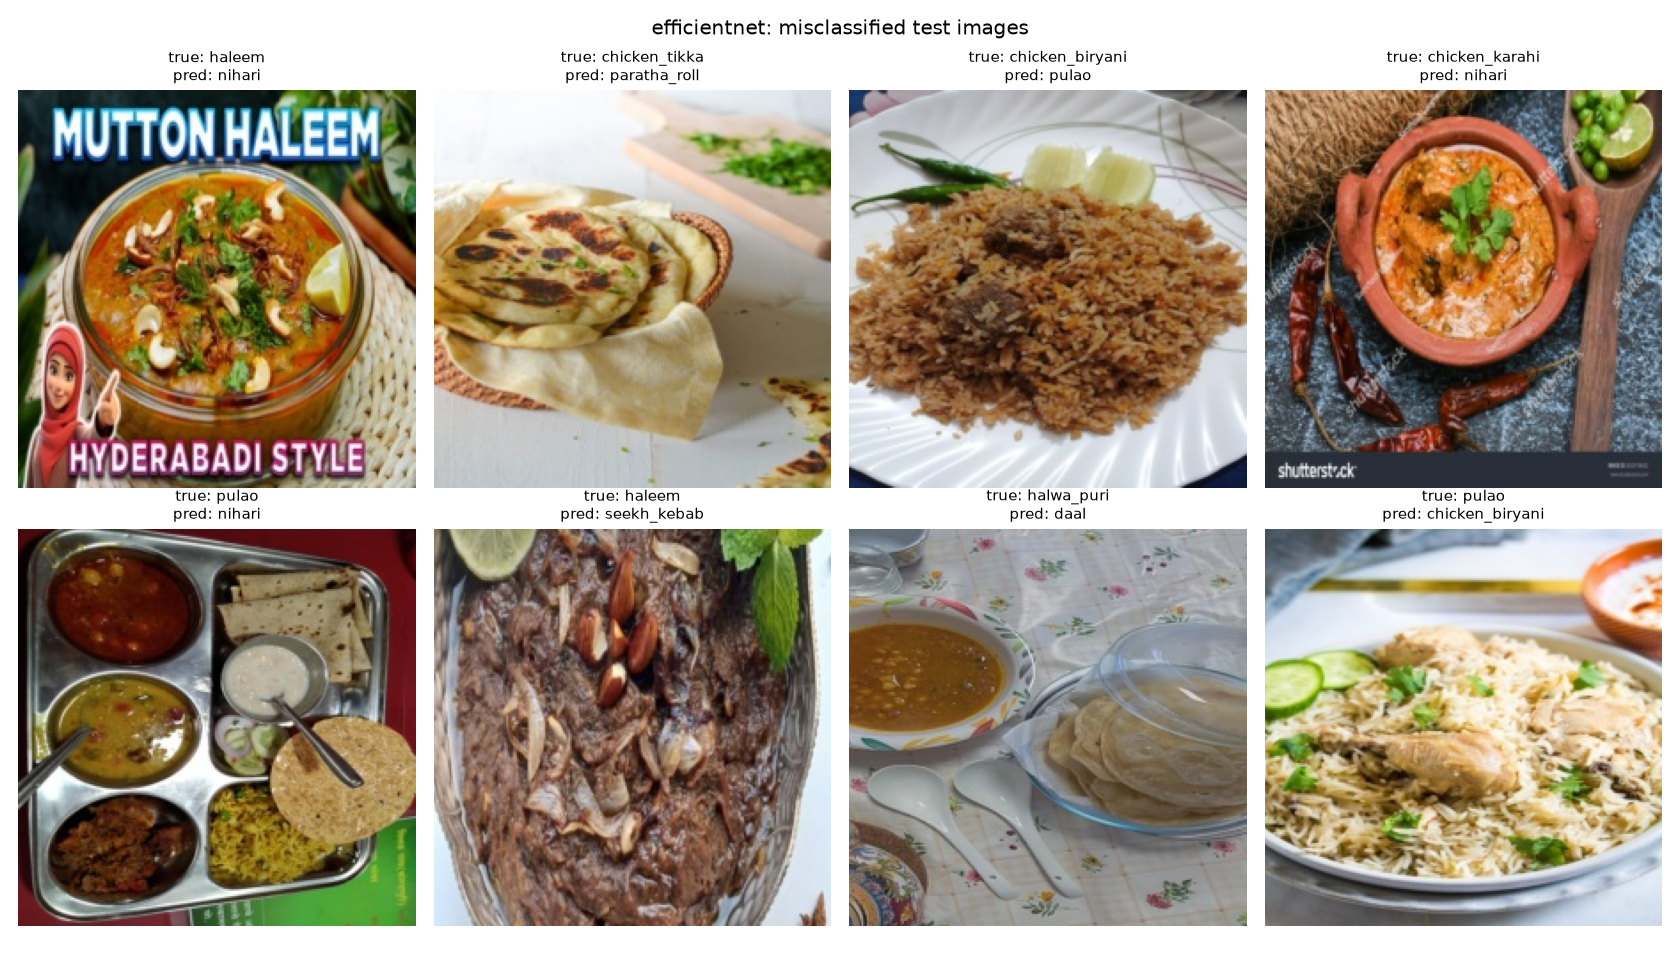
\includegraphics[width=0.95\textwidth]{failures_efficientnet.png}
  \caption{Misclassified test images (EfficientNet-B0), with true and
  predicted dish in each title.}
  \label{fig:failures}
\end{figure}

Reading the figure from left to right, top row first:
\begin{enumerate}
  \item True \texttt{haleem}, predicted \texttt{nihari}: a thick orange-brown
        stew in a glass bowl topped with cashews, fried onions and lime, with
        a large ``MUTTON HALEEM'' text overlay and a cartoon figure.
  \item True \texttt{chicken\_tikka}, predicted \texttt{paratha\_roll}: the
        photo shows flatbreads in a basket with chopped herbs and no visible
        chicken, so the label does not match the main content.
  \item True \texttt{chicken\_biryani}, predicted \texttt{pulao}: a plate of
        brown rice with pieces of meat, green chillies and lemon wedges,
        which looks like a pulao-style rice dish.
  \item True \texttt{chicken\_karahi}, predicted \texttt{nihari}: a red-orange
        curry in a clay pot with dried red chillies and a stock-photo
        watermark.
  \item True \texttt{pulao}, predicted \texttt{nihari}: a metal tray with
        several small bowls (curries, dal, yoghurt), flatbread and papad, and
        only a small portion of yellow rice.
  \item True \texttt{haleem}, predicted \texttt{seekh\_kebab}: a close-up of a
        dark brown, mashed-looking dish topped with almonds, fried onions and
        mint; no skewers are visible.
  \item True \texttt{halwa\_puri}, predicted \texttt{daal}: a bowl of yellow
        dal sits beside a glass dish of flatbreads, and the dal is the most
        prominent item on the table.
  \item True \texttt{pulao}, predicted \texttt{chicken\_biryani}: white rice
        with a chicken piece, herbs and cucumber slices, which is close to how
        a biryani plate looks.
\end{enumerate}
These are descriptions of what is visible, not tested explanations of the
model's errors.

\subsection{Bias check}
{\sloppy
The dataset contains photos of food only and no people, so demographic
subgroups do not apply. The closest available subgroups are the image
\emph{source} and \emph{setting} recorded in \texttt{data/processed/split.csv}.
Table~\ref{tab:subgroups} shows test accuracy by group, from
\texttt{results/\allowbreak bias\_\allowbreak baseline\_\allowbreak subgroups.csv} and
\texttt{results/\allowbreak bias\_\allowbreak efficientnet\_\allowbreak subgroups.csv}.\par}

\begin{table}[H]
  \centering
  \begin{tabular}{|l|l|r|r|r|}
    \hline
    \textbf{Group type} & \textbf{Group} & \textbf{Images} &
    \textbf{Baseline acc.} & \textbf{EfficientNet acc.} \\ \hline
    Source  & Bing       & 485 & 0.466 & 0.761 \\ \hline
    Source  & Kaggle     & 156 & 0.641 & 0.917 \\ \hline
    Setting & home       &  86 & 0.512 & 0.779 \\ \hline
    Setting & restaurant & 111 & 0.486 & 0.757 \\ \hline
    Setting & unknown    & 444 & 0.514 & 0.813 \\ \hline
  \end{tabular}
  \caption{Test accuracy by source and setting.}
  \label{tab:subgroups}
\end{table}

Both models score higher on Kaggle images than on Bing images (EfficientNet
0.917 versus 0.761). We cannot say why from these results; one possible
reason is that the Kaggle photos are more uniform, but this was not tested.
The Kaggle images cover only four dishes (samosa, pakora, daal and paratha
roll), which are among the best-recognised classes in Table~\ref{tab:f1}
(EfficientNet F1 0.81 to 0.94), so this gap is partly a dish effect and not a
clean source effect. We did not compare Bing and Kaggle within the same dish.
Setting differences are small and mixed, and 444 of the 641 test images
have setting \texttt{unknown}, so the home and restaurant groups say little.
We also split test images into dark, medium and bright thirds by brightness
(rows with group type \texttt{brightness} in the same two subgroup files).
EfficientNet accuracy was 0.813, 0.808 and 0.776 and the baseline's was
0.472, 0.531 and 0.523, so there is no consistent brightness effect.

\textbf{Limits.} The test set has only 641 images, so small groups (for
example Kaggle with 156 and home with 86) give noisy estimates. Scraped
images can contain watermarks or wrong labels, and the setting label is
unknown for most images. These results show where the models differ, not
proven causes.

\subsection{Comparison and Sample Predictions}
EfficientNet-B0 with ImageNet transfer learning reached $0.7988$ test accuracy
and $0.7785$ macro F1, against $0.5086$ and $0.4700$ for the from-scratch
baseline, and it achieved a higher F1 on every single dish. Figure~\ref{fig:sample-preds}
shows a $3 \times 4$ grid of test-set predictions from EfficientNet-B0
(\texttt{report/figures/sample\_predictions.png}, generated by
\texttt{src/sample\_predictions.py} with 8 correct and 4 misclassified test
images sampled using \texttt{random.seed(42)}). Each tile displays the ground
truth, the predicted dish, and the top-1 softmax confidence, coloured green
for correct predictions and red for errors.

\begin{figure}[H]
  \centering
  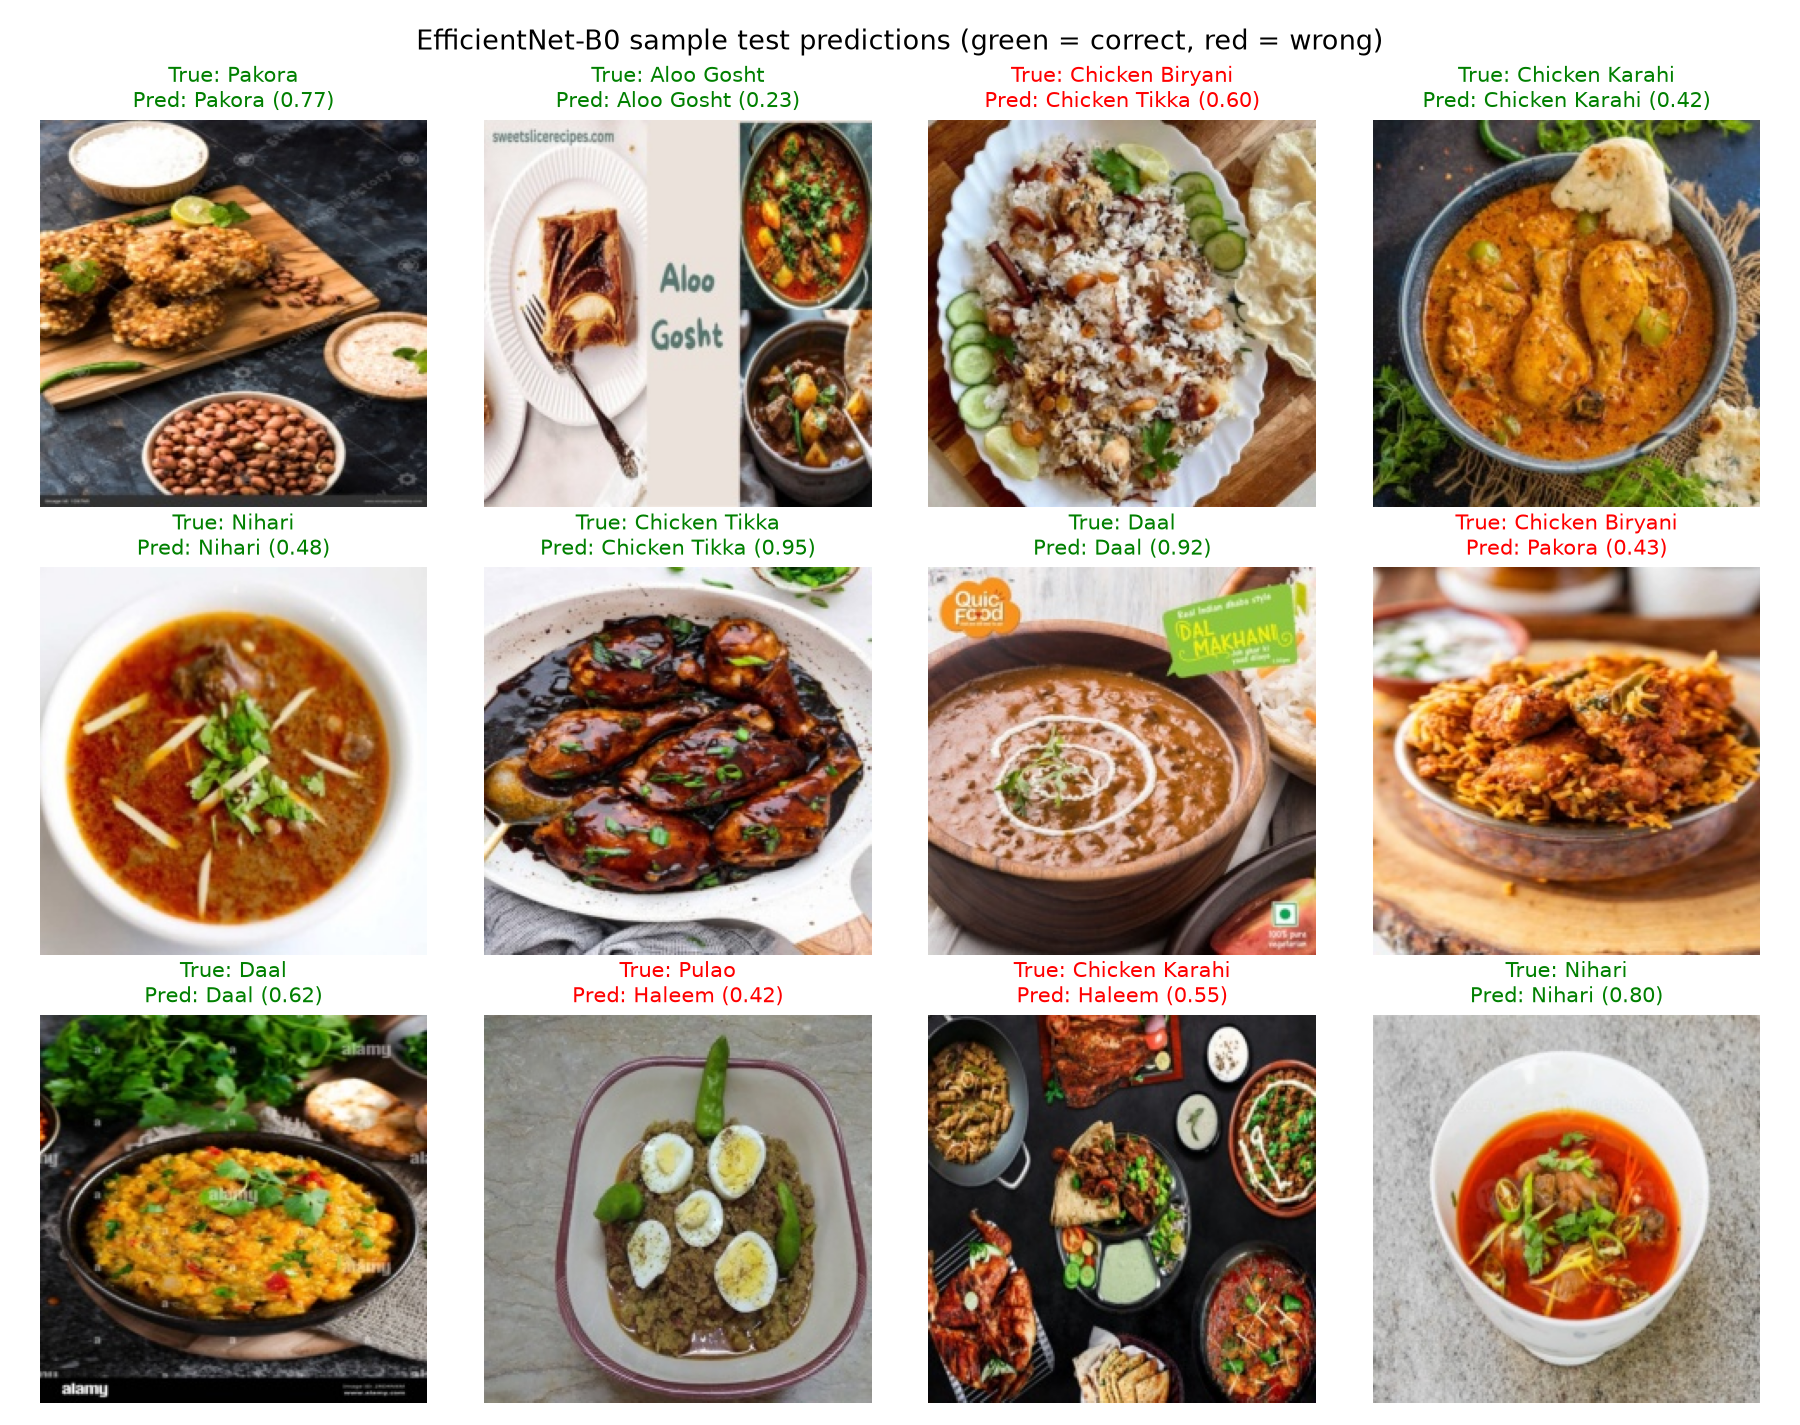
\includegraphics[width=0.95\textwidth]{sample_predictions.png}
  \caption{Sample test-set predictions from EfficientNet-B0
  (\texttt{report/figures/sample\_predictions.png}): 8 correct (green) and 4
  misclassified (red) test images sampled with seed 42, showing true dish,
  predicted dish, and top-1 confidence.}
  \label{fig:sample-preds}
\end{figure}


\section{Application and Calorie Module}
\IfFileExists{phase5_app.tex}{% Application report section -- written by Huzaifa.
% Included from main.tex inside \section{Application and Calorie Module}.
% Numbers come from results/ood_thresholds.json, ood_val.csv, ood_test.csv and ood_probe.csv.
\subsection{Web Application Architecture and Interface}

The trained EfficientNet-B0 is served through a web application with two parts:
a Python backend that runs the model, and a browser frontend where the user
uploads a photo. Both run locally on a laptop; hosting was out of scope for this
deliverable. The backend lives in \texttt{app/backend/} and the frontend in
\texttt{app/frontend/}. A single command, \texttt{./run.sh}, starts both.

\subsubsection{Backend}
The backend is a FastAPI application (\texttt{app/backend/main.py}) with the
endpoints in Table~\ref{tab:endpoints}.

\begin{table}[H]
  \centering
  \small
  \begin{tabular}{|l|p{10.2cm}|}
    \hline
    \textbf{Endpoint} & \textbf{Purpose} \\ \hline
    \texttt{GET /health} & Status, number of classes, thresholds and whether the
      calorie module is available. \\ \hline
    \texttt{GET /dishes} & The 14 dish names. \\ \hline
    \texttt{POST /predict} & Takes an image (at most 10~MB) and an optional
      \texttt{portion} between 0.25 and 4. Returns the top 3 dishes with
      confidence, an \texttt{in\_scope} flag with a \texttt{reason} when the photo
      is rejected, and the calorie range. \\ \hline
    \texttt{GET /calories} & Calorie range for a chosen dish and portion, without
      running the model. Used after a user correction. \\ \hline
    \texttt{POST /feedback} & Stores the dish a user says the photo really shows
      (one of the 14 dishes, or \texttt{none}). \\ \hline
  \end{tabular}
  \caption{Backend endpoints.}
  \label{tab:endpoints}
\end{table}

\texttt{app/backend/model\_service.py} loads
\texttt{checkpoints/efficientnet\_best.pt} once, when the server starts, and keeps
the model in memory in evaluation mode. Each uploaded image is opened with Pillow,
rotated according to its EXIF orientation (phone photos often store rotation
there), converted to RGB, and passed through the same validation transform used
in training (\texttt{eval\_transforms()} in \texttt{src/dataset.py}: resize to
$224 \times 224$ and ImageNet mean and standard deviation). Reusing that function
means the application cannot drift away from the preprocessing the model was
evaluated with. The softmax output gives the top 3 classes, and the 1280-value
feature vector in front of the classifier is kept for the out-of-scope check
below. An unreadable file returns status 400, a file over 10~MB returns 413, and
a \texttt{portion} outside 0.25 to 4 returns 422.

\subsubsection{Out-of-scope check}
A classifier with 14 outputs must name one of them even for a photo that is not
one of the dishes. In our probe photos (below), a close-up photo of an arm
reached a top-1 confidence of 0.473, above the 0.45 confidence threshold chosen on
the validation set, so confidence alone would have accepted it as a dish. The application therefore rejects a photo if
either of two checks fails.
\begin{enumerate}
  \item \textbf{Confidence.} The top softmax probability must be at least
        $0.45$ (the threshold chosen on the validation set, described in the
        confidence threshold subsection below).
  \item \textbf{Similarity.} The cosine similarity between the photo's feature
        vector and the nearest of 14 dish centroids must be at least
        $0.4059$. The centroids are the mean feature vectors of the training
        images of each dish (\texttt{results/ood\_reference.npz}). The threshold
        was chosen on the validation set so that 88\% of correctly classified
        validation photos still pass; the script \texttt{src/ood\_analysis.py}
        computes it and writes \texttt{results/ood\_thresholds.json}.
\end{enumerate}
With both checks the model answers 75.7\% of the test images, with 88.2\%
accuracy on the answered ones (\texttt{results/ood\_test.csv}). A rejected photo
gets no calorie estimate: the interface says that the photo is not one of the
supported dishes and shows the 14 dishes.

We tested the rejection on 30 photos that are not dishes
(\texttt{results/ood\_probe.csv}): 26 random scenery and object photos from a free
photo site, and four photos we supplied (three portraits and the arm close-up).
29 of the 30 were rejected, all by the similarity check; the one that passed was a
photo of a desert dune, whose similarity (0.407) was barely above the threshold.
The set is small, informal and mostly scenery, so it shows that the check works
on common cases, not that it catches every non-dish photo. Tightening the
threshold would reject more non-dish photos but also more real dishes, because
the similarity threshold is a trade-off.

\subsubsection{User feedback}
Under every answer the interface asks ``Is this correct?''. \emph{Yes} confirms the
answer. \emph{No} opens a picker that lists the model's other guesses first, then
all 14 dishes and a ``None of these'' option; choosing a dish immediately shows
that dish with its calories, and the user can change the answer again. Photos
rejected as out of scope can be corrected in the same way if the dish was
wrongly rejected.

Each answer is saved by the backend as one line in
\texttt{feedback/corrections.jsonl} together with the photo. A record holds an
identifier, a UTC timestamp, the image file and its SHA-256 hash, the predicted
label, confidence and top three guesses, the in-scope flag and reason, the
corrected label and whether the model was right. The backend runs the model
itself on the posted photo, so the stored prediction cannot be edited by the
client. Photos are re-saved as JPEG, which drops EXIF data such as location, and
the \texttt{feedback/} folder is excluded from Git because it holds user photos.
The records can be used later to evaluate or retrain the model.

\subsubsection{Tests}
Three test files cover the application. \texttt{tests/test\_api.py} (six tests)
checks the health and dish endpoints, the shape of a prediction, and that a
non-image file, a bad portion and a flat colour image are handled correctly.
\texttt{tests/test\_ood.py} (six tests) checks the rejection logic.
\texttt{tests/test\_feedback.py} (five tests) checks the calories and feedback
endpoints; these write to a temporary folder. The tests that load the model are
skipped when the weights file is absent.

\subsubsection{Frontend}
The frontend is a React application built with Vite
(\texttt{app/frontend/src/}). During development it forwards requests under
\texttt{/api} to the backend on port 8000. Its main parts are:
\begin{itemize}
  \item \textbf{Upload and camera:} drag and drop, a file picker, or a photo taken
        with the device camera, with a clear message when camera permission is
        blocked.
  \item \textbf{Result card:} the dish name, the confidence, and two tiles with
        the typical energy and the likely range, followed by the serving
        description and an expandable list of the sources behind the numbers.
  \item \textbf{Portion picker:} Small ($0.75\times$), Regular ($1\times$), Large
        ($1.5\times$) and Double ($2\times$). Choosing one asks the backend for
        the new calorie values, so the numbers always come from the server.
  \item \textbf{Top guesses:} the three most likely dishes with their
        confidences, drawn as a menu with dotted leaders.
  \item \textbf{Feedback and picker:} the ``Is this correct?'' control and the
        out-of-scope screen described above.
  \item \textbf{Session history:} the last six photos and their results, kept in
        memory only.
\end{itemize}
The visual design follows an organic editorial style: a cream and deep green
palette with terracotta accents, a high-contrast serif for headlines, a large
food photograph in the opening section, and a calorie card that overlaps the
photo. There is a light and a dark theme. The interface uses short transitions
(scroll reveals, a slight parallax on the opening photo, counting numbers and
growing bars), which are switched off when the user's system asks for reduced
motion. The opening photo is by Shreyak Singh from Unsplash.

\subsubsection{Interface examples}
Figure~\ref{fig:app-landing} shows the opening screen and Figure~\ref{fig:app-result}
a confident prediction for a chicken biryani photo from the test set.
Figure~\ref{fig:app-feedback} shows the picker that opens when the user presses
\emph{No}. Figure~\ref{fig:app-oos} shows a photo that is not a dish, here a flag,
which the application rejects without a calorie estimate and with the dish list
instead.

\begin{figure}[H]
  \centering
  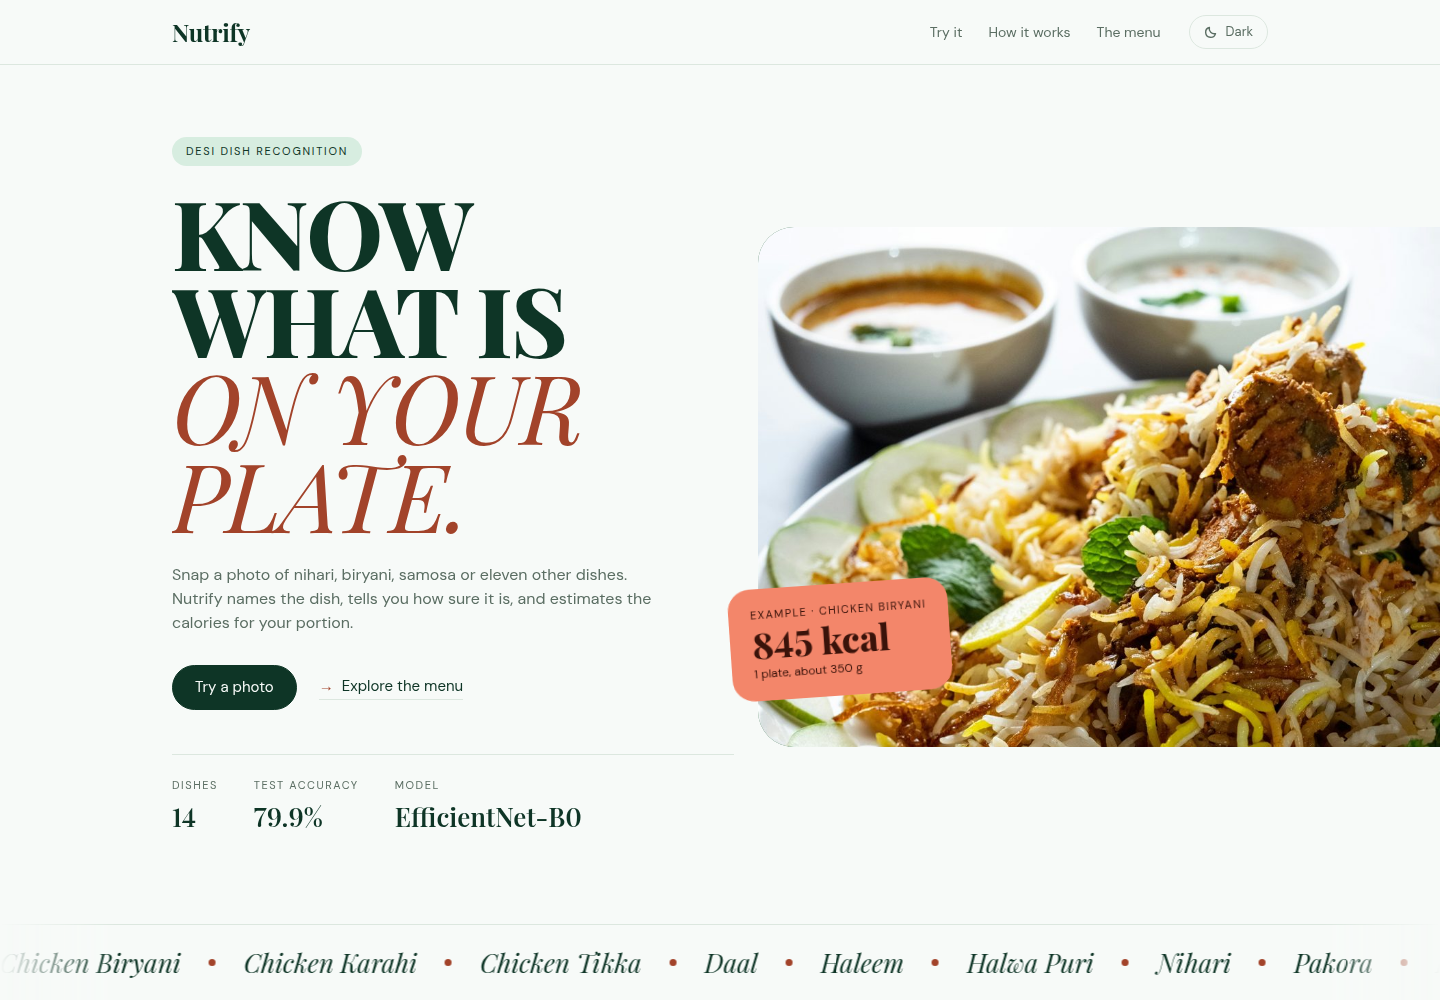
\includegraphics[width=0.95\textwidth,height=0.5\textheight,keepaspectratio]{app_landing.png}
  \caption{Opening screen of the application (light theme).}
  \label{fig:app-landing}
\end{figure}

\begin{figure}[H]
  \centering
  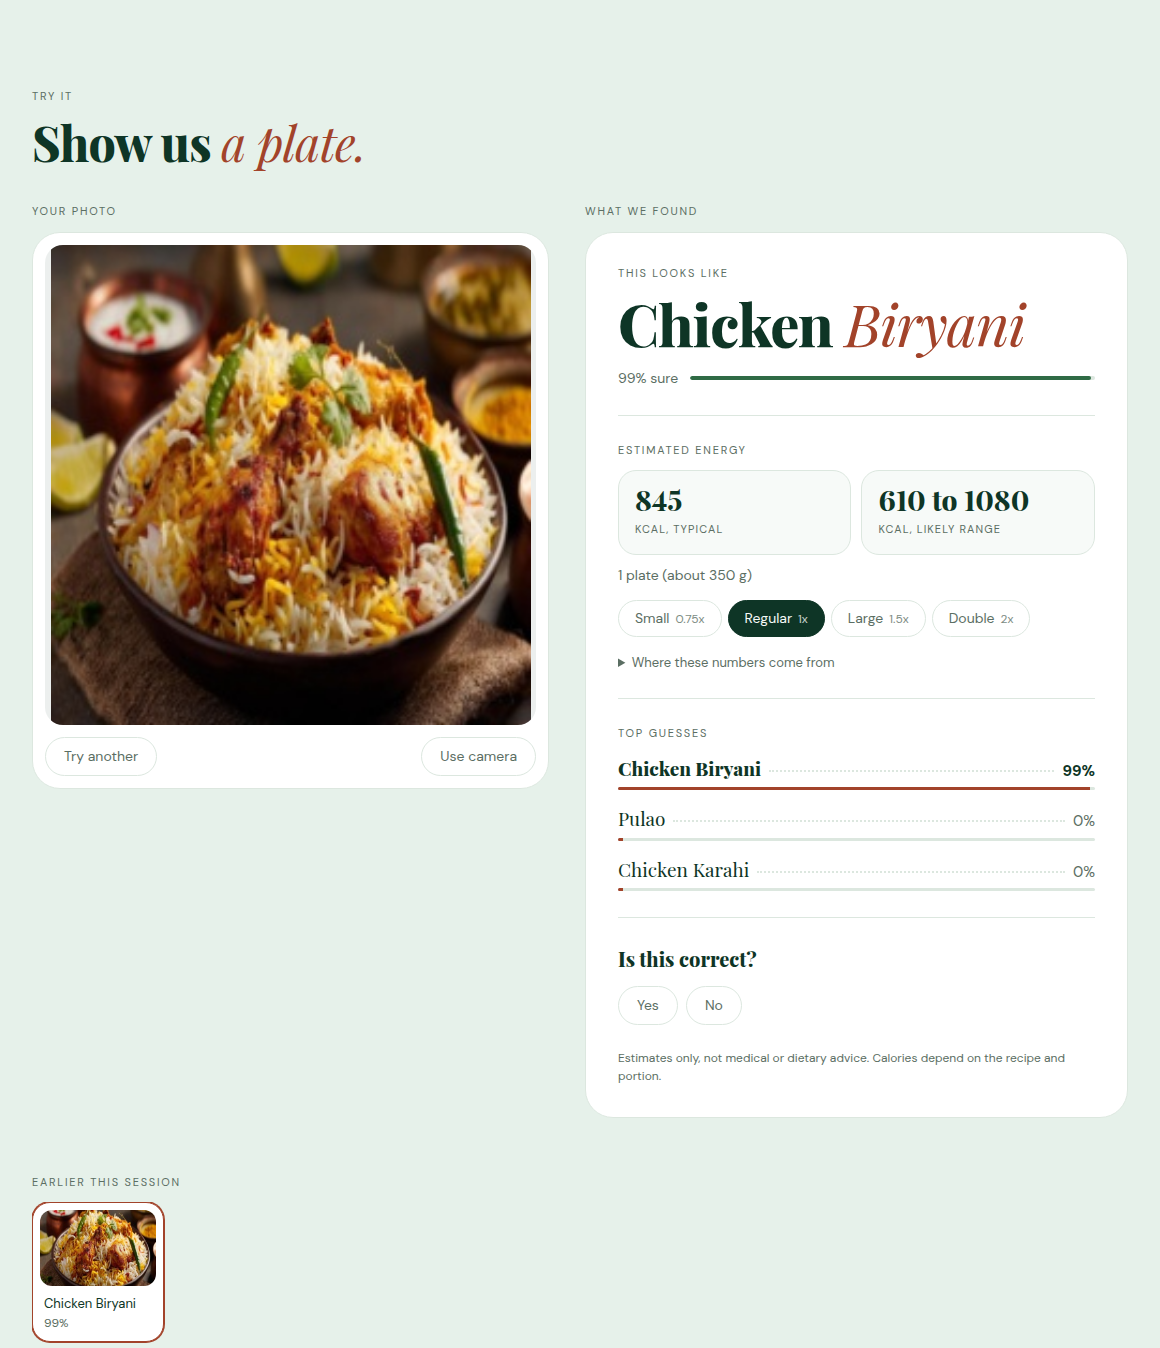
\includegraphics[width=0.8\textwidth,height=0.55\textheight,keepaspectratio]{app_screenshot.png}
  \caption{Confident prediction: dish, confidence, calorie tiles, portion pills,
  top three guesses, the feedback question and session history.}
  \label{fig:app-result}
\end{figure}

\begin{figure}[H]
  \centering
  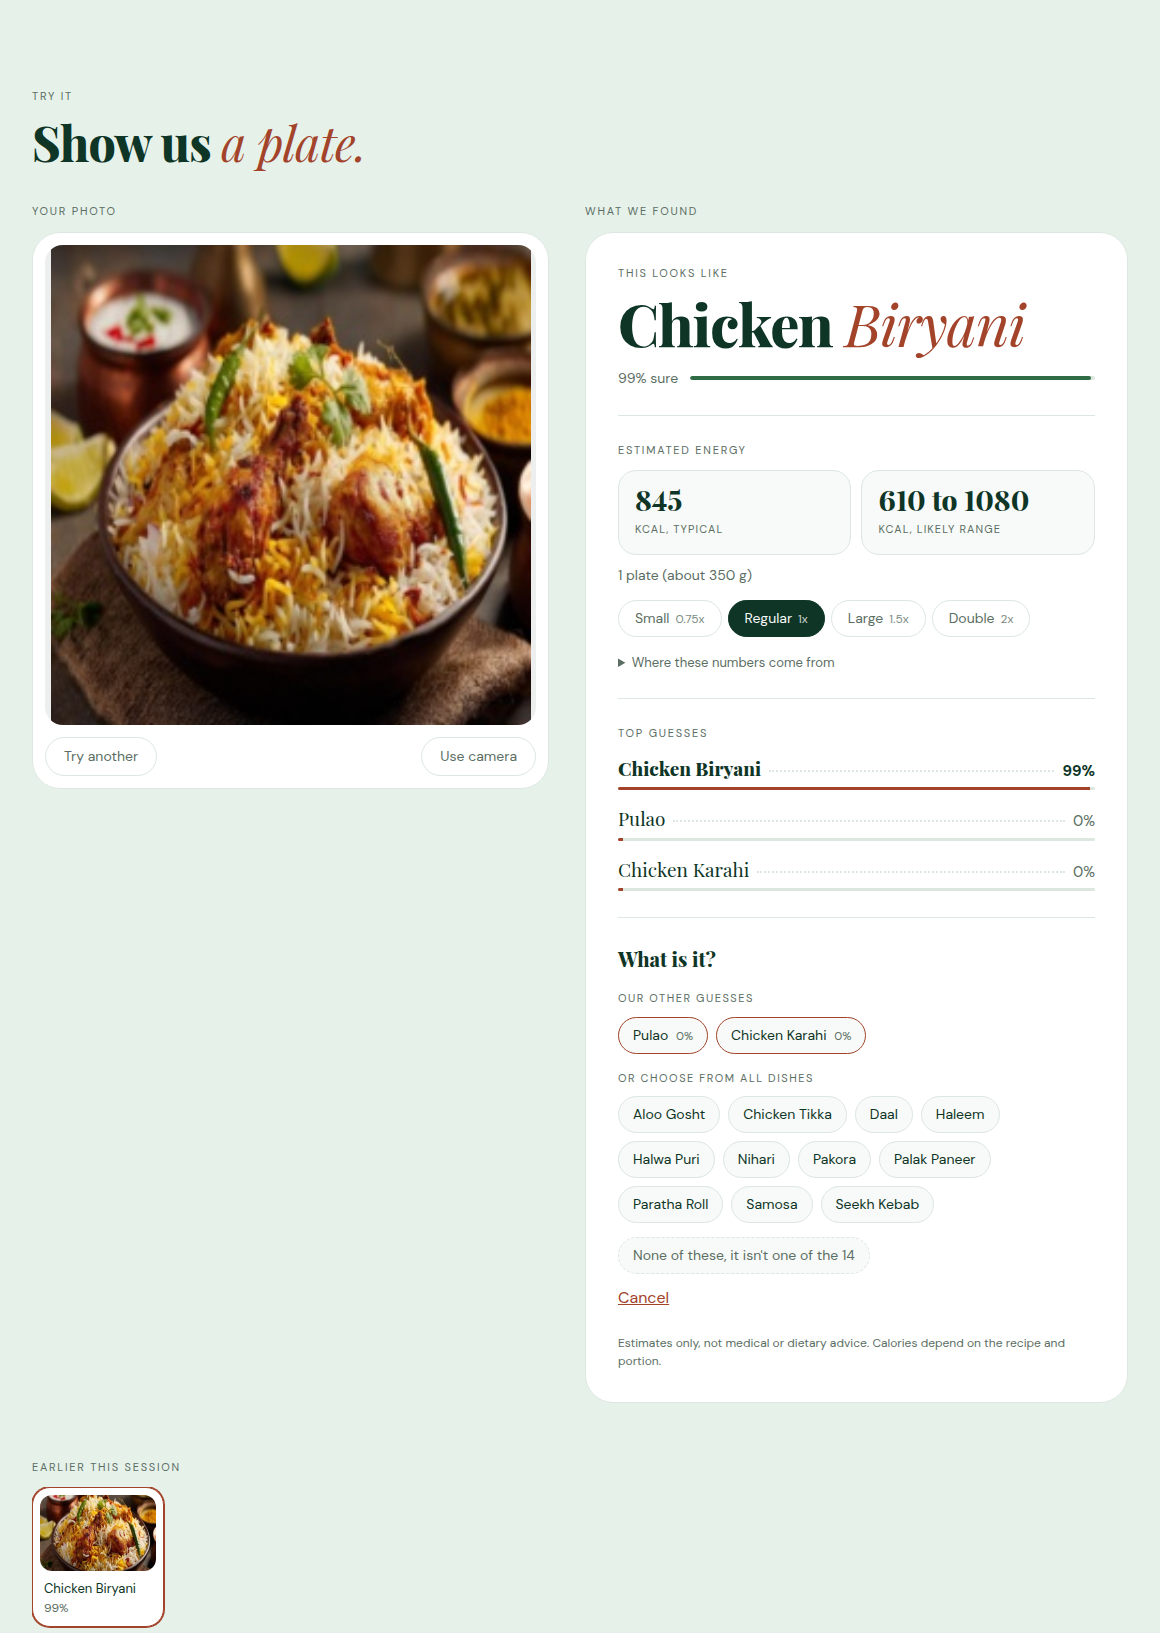
\includegraphics[width=0.8\textwidth,height=0.55\textheight,keepaspectratio]{app_feedback.png}
  \caption{After pressing \emph{No}: the user picks the right dish from the model's
  other guesses or from all 14 dishes, or chooses ``None of these''.}
  \label{fig:app-feedback}
\end{figure}

\begin{figure}[H]
  \centering
  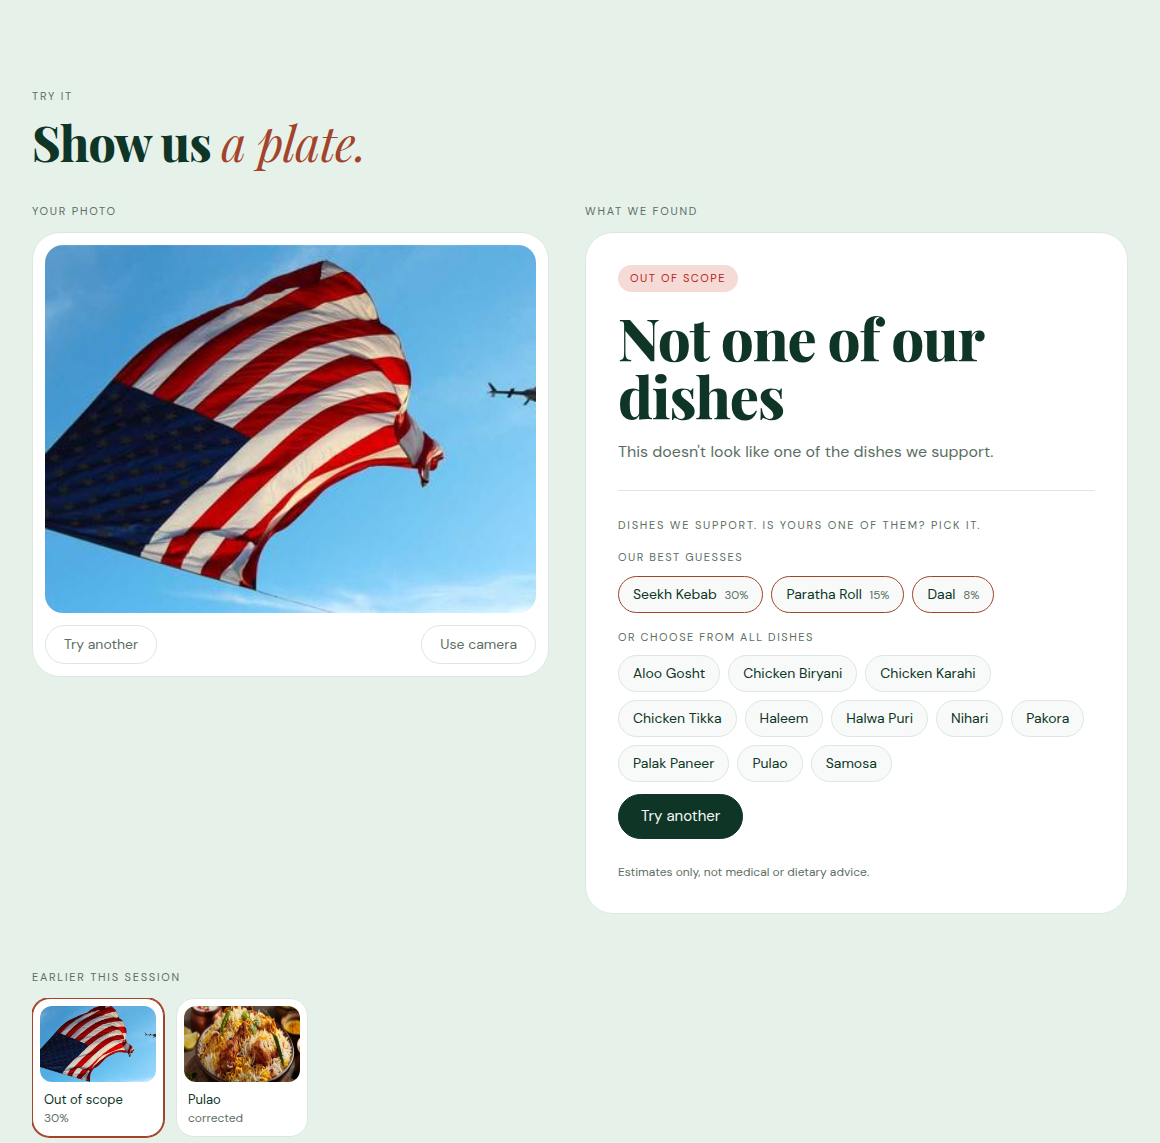
\includegraphics[width=0.8\textwidth,height=0.55\textheight,keepaspectratio]{app_out_of_scope.png}
  \caption{A photo that is not a dish is rejected: no calories, the supported
  dishes, and the option to pick the right dish if the rejection was wrong.}
  \label{fig:app-oos}
\end{figure}

The application does not detect the portion size from the photo. The user
chooses it, and the calorie numbers are estimates from recipes and food
composition tables (see the calorie and threshold limitations below).
}{}
\subsection{Calorie Estimation Module}

Pakistan currently lacks an up-to-date national food composition table for
cooked composite dishes~\cite{soomro2024matiari}. Rather than training a black-box
regressor to guess calories from pixels, Nutrify maps each recognised dish
through \texttt{src/calories.py} and \texttt{src/calories.json} to a
deterministic per-serving calorie range (low, typical, and high), which is
scaled linearly by the user's selected portion multiplier.

\paragraph{How each range was obtained.}
Because standard food composition tables list raw ingredients rather than
prepared Pakistani dishes, we constructed recipe-based estimates for one
standard serving of each of the 14 dishes. Primary ingredient energies are
taken from Table~1 of the Indian Food Composition Tables 2017 (IFCT
2017)~\cite{longvah2017ifct}, converted from kilojoules to kilocalories using
$1\text{ kJ} = 0.239\text{ kcal}$ (IFCT computes metabolisable energy using
Atwater factors, General Information, pp.~xxi--xxii). Cooking fats, dairy, and
other staple items not listed in the same form in IFCT (sunflower oil T508 at
$899\text{ kcal/100 g}$, butter ghee T506 at $878\text{ kcal/100 g}$, whole-milk
plain yogurt L520 at $79\text{ kcal/100 g}$, white sugar I502 at
$394\text{ kcal/100 g}$, gram flour A504 at $353\text{ kcal/100 g}$, and fresh
single cream L519 at $193\text{ kcal/100 g}$) are taken from McCance and
Widdowson's Composition of Foods Integrated Dataset (CoFID)~\cite{cofid2021},
as compiled in the open-access Indian Nutrient Databank
(INDB)~\cite{vijayakumar2024indb}.

For each dish, the \emph{typical} value sums the edible ingredient energies for
a home-style or standard restaurant serving, rounded to the nearest
$5\text{ kcal}$. Spices, salt, water, and light garnishes contribute negligible
energy and are omitted; cooking changes moisture content rather than total
energy, and frying oil is counted as the estimated amount absorbed or eaten
rather than the full pan volume. The \emph{low} and \emph{high} values
represent a leaner recipe version (less oil or ghee and leaner meat cuts, such
as skinless chicken breast N003 at $168\text{ kcal/100 g}$ or goat legs O003 at
$160\text{ kcal/100 g}$) and a richer recipe version (more oil or ghee, fattier
cuts such as chicken thigh N002 at $200\text{ kcal/100 g}$ or beef shoulder
O025 at $212\text{ kcal/100 g}$, and a larger main-ingredient portion).
Table~\ref{tab:calories} lists the 14 dishes, their standard serving
descriptions, and their low, typical, and high kilocalorie values from
\texttt{src/calories.json}.

\begin{table}[H]
  \centering
  \small
  \begin{tabular}{|p{4.3cm}|p{4.8cm}|r|r|r|}
    \hline
    \textbf{Dish} & \textbf{Standard serving} & \textbf{Low} & \textbf{Typical} & \textbf{High} \\
    \hline
    Aloo Gosht (\texttt{aloo\_gosht}) & 1 bowl (about 300 g) & 355 & 540 & 700 \\
    Chicken Biryani (\texttt{chicken\_biryani}) & 1 plate (about 350 g) & 610 & 845 & 1080 \\
    Chicken Karahi (\texttt{chicken\_karahi}) & 1 bowl (about 250 g) & 385 & 580 & 770 \\
    Chicken Tikka (\texttt{chicken\_tikka}) & 4 pieces (about 150 g cooked) & 320 & 400 & 515 \\
    Daal (\texttt{daal}) & 1 bowl (about 250 g) & 195 & 295 & 405 \\
    Haleem (\texttt{haleem}) & 1 bowl (about 300 g) & 365 & 600 & 835 \\
    Halwa Puri (\texttt{halwa\_puri}) & 2 puri, 1 small bowl halwa, a little chana (about 250 g) & 620 & 810 & 1085 \\
    Nihari (\texttt{nihari}) & 1 bowl (about 300 g) & 340 & 585 & 800 \\
    Pakora (\texttt{pakora}) & 6 pieces (about 100 g) & 210 & 295 & 405 \\
    Palak Paneer (\texttt{palak\_paneer}) & 1 bowl (about 250 g) & 235 & 355 & 495 \\
    Paratha Roll (\texttt{paratha\_roll}) & 1 roll (about 200 g) & 410 & 545 & 710 \\
    Pulao (\texttt{pulao}) & 1 plate (about 300 g) & 420 & 560 & 715 \\
    Samosa (\texttt{samosa}) & 2 samosas (about 130 g) & 305 & 405 & 510 \\
    Seekh Kebab (\texttt{seekh\_kebab}) & 2 kebabs (about 120 g cooked) & 195 & 315 & 400 \\
    \hline
  \end{tabular}
  \caption{Per-serving calorie estimates in kcal for the 14 dishes, from \texttt{src/calories.json}.}
  \label{tab:calories}
\end{table}

\subsection{Confidence Threshold and Non-Dish Check}

Because a 14-way softmax layer always assigns probabilities that sum to $1$,
the classifier will output a dish name even when given a blurry photo, an
ambiguous dish, or an image that does not contain food at all. To prevent the
application from presenting low-confidence guesses as definite answers,
\texttt{src/confidence\_analysis.py} selects a rejection threshold $\tau$ on
the 640-image validation set. When the top softmax probability falls below
$\tau$, the application withholds the dish decision and the calorie estimate. (In the
final application such a photo is reported as out of scope, and a second
feature-similarity check was added; see the application section above.)

\paragraph{Validation sweep and test evaluation.}
We swept $\tau$ from $0.30$ to $0.90$ in steps of $0.05$ on the validation set
(\texttt{results/confidence\_val.csv}) and applied the selection rule: choose
the smallest threshold achieving at least $0.90$ accuracy on accepted images
while keeping coverage at or above $0.50$. Table~\ref{tab:confidence-val}
shows the full validation sweep. The smallest qualifying threshold is
$\tau = 0.45$ (\texttt{results/confidence\_threshold.json}), which achieves
$0.9173$ validation accuracy at $0.8313$ coverage. Applied once to the 641
held-out test predictions (\texttt{results/confidence\_test.csv}),
$\tau = 0.45$ yields a test coverage of \textbf{0.8456} and raises test
accuracy on accepted images from $0.7988$ (unthresholded) to \textbf{0.8727}.

\begin{table}[H]
  \centering
  \small
  \begin{tabular}{|r|r|r|}
    \hline
    \textbf{Threshold ($\tau$)} & \textbf{Val.\ coverage} & \textbf{Val.\ accuracy (accepted)} \\
    \hline
    0.30 & 0.9375 & 0.8717 \\
    0.35 & 0.9078 & 0.8847 \\
    0.40 & 0.8750 & 0.8964 \\
    \textbf{0.45} & \textbf{0.8313} & \textbf{0.9173} \\
    0.50 & 0.7828 & 0.9301 \\
    0.55 & 0.7469 & 0.9393 \\
    0.60 & 0.7109 & 0.9560 \\
    0.65 & 0.6781 & 0.9608 \\
    0.70 & 0.6312 & 0.9653 \\
    0.75 & 0.5828 & 0.9705 \\
    0.80 & 0.5078 & 0.9815 \\
    0.85 & 0.4250 & 0.9890 \\
    0.90 & 0.3172 & 0.9951 \\
    \hline
  \end{tabular}
  \caption{Validation coverage and accuracy on accepted images across candidate
  thresholds (\texttt{results/confidence\_val.csv}). Bold marks the selected
  threshold $\tau = 0.45$, which achieves $0.8456$ coverage and $0.8727$
  accuracy on the test set (\texttt{results/confidence\_test.csv}).}
  \label{tab:confidence-val}
\end{table}

\paragraph{Informal non-dish check.}
To see how the threshold behaves on out-of-distribution inputs, we ran an
informal check on 6 non-dish photos (\texttt{results/non\_dish\_check.csv}),
shown in Table~\ref{tab:non-dish}. Because there are only 6 images, this is a
qualitative sanity check rather than a statistical benchmark. Four of the 6
images had top softmax confidence between $0.25$ and $0.35$ and were correctly
rejected as \texttt{Not sure}. The remaining two images (a selfie in a grey
T-shirt with a phone at $0.45$ and a selfie in a grey T-shirt at $0.58$) met or
exceeded the $0.45$ threshold and were wrongly accepted as \texttt{Samosa}.

\begin{table}[H]
  \centering
  \small
  \begin{tabular}{|l|r|l|}
    \hline
    \textbf{Image description} & \textbf{Top confidence} & \textbf{App answer ($\tau = 0.45$)} \\
    \hline
    face photo blue shirt & 0.30 & Not sure \\
    Nike logo & 0.35 & Not sure \\
    screen with code & 0.25 & Not sure \\
    selfie grey T-shirt with phone & 0.45 & Samosa \\
    selfie grey T-shirt & 0.58 & Samosa \\
    selfie flexing & 0.33 & Not sure \\
    \hline
  \end{tabular}
  \caption{Informal check on 6 non-dish images (\texttt{results/non\_dish\_check.csv}).}
  \label{tab:non-dish}
\end{table}

\subsection{Calorie and Threshold Limitations}

Several methodological limitations apply to the calorie estimates and the
confidence filter:
\begin{itemize}
  \item \textbf{Recipe estimates, not measurements:} All values in
        \texttt{src/calories.json} are recipe-based calculations from food
        composition tables, not bomb-calorimetry measurements of the photographed
        meal, and they are for general informational use rather than medical or
        clinical dietary advice.
  \item \textbf{Assumed serving sizes and unmeasured portions:} The standard
        serving weight and every ingredient weight in a recipe are fixed
        assumptions. The system does not detect food volume, depth, or plate
        scale from the photo; portion adjustments rely entirely on the user's
        chosen multiplier.
  \item \textbf{Lean and rich recipes, not statistical intervals:} The
        \texttt{kcal\_low} and \texttt{kcal\_high} bounds represent a lean recipe
        variant (less oil or ghee, leaner meat cut) and a rich recipe variant
        (more oil or ghee, fattier cut, larger main-ingredient weight), not
        statistical confidence intervals or standard deviations across kitchens.
  \item \textbf{Cooked poultry weights in IFCT 2017:} IFCT 2017 reports nutrient
        values for raw edible foods \emph{except} for poultry and egg (General
        Information, p.~xx). Accordingly, the chicken weights in our recipes
        (\texttt{chicken\_biryani}, \texttt{chicken\_karahi},
        \texttt{chicken\_tikka}, \texttt{paratha\_roll}, and \texttt{pulao})
        refer to cooked boneless skinless chicken breast (N003,
        $168\text{ kcal/100 g}$) or thigh (N002, $200\text{ kcal/100 g}$),
        whereas red meat, grains, pulses, and vegetables are entered as raw
        edible weights.
  \item \textbf{Omission of IFCT ``chicken, leg, skinless'':} The IFCT 2017
        entry for skinless chicken leg reports an energy of about
        $384\text{ kcal/100 g}$, which is inconsistent with its own reported
        protein and fat content under Atwater conversion; we therefore excluded
        that entry and used only breast (N003) and thigh (N002).
  \item \textbf{Why INDB cooked-dish totals were used only as a cross-check:}
        The Indian Nutrient Databank~\cite{vijayakumar2024indb} includes
        calculated recipes for several Indian dishes (for example Mutton biryani
        ASC122 at $396\text{ kcal}$ per plate, Dal makhani OSR139 at
        $262\text{ kcal}$ per bowl, Spinach paneer ASC215 at $230\text{ kcal}$
        per bowl, and Plain pulao ASC114 at $432\text{ kcal}$ per plate). We did
        not adopt INDB's cooked-dish totals directly because INDB counts all
        frying oil in a recipe as consumed and does not apply cooking yield
        factors; we used INDB only to source UK CoFID~\cite{cofid2021}
        ingredient values and as a sanity cross-check.
  \item \textbf{Closed-set classifier and imperfect rejection:} Because the
        network is trained strictly on 14 classes, it always picks one of those
        14 dishes. The $0.45$ confidence threshold catches most uncertain or
        non-dish photos (4 of 6 in our informal check), but out-of-distribution
        images can still produce a softmax peak at or above $0.45$ and be
        accepted as one of the 14 dishes.
\end{itemize}



\section{Discussion and Limitations}

\paragraph{Why samples fail: look-alike dishes.}
The confusion matrices and per-pair error counts
(\texttt{results/bias\_efficientnet\_confusions.csv}) show that visual
similarity between related South Asian preparations is the primary source of
classification errors. For EfficientNet-B0, the most frequent confusion pair is
\texttt{pulao} predicted as \texttt{chicken\_biryani} (7 test images) and
\texttt{chicken\_biryani} predicted as \texttt{pulao} (6 images); both are
spiced rice dishes served with chicken pieces, herbs, and sliced garnishes, and
they are reflected in the two lowest per-dish test F1 scores (\texttt{pulao}
$0.604$, \texttt{chicken\_biryani} $0.649$). Similarly, thick brown or
red-orange gravies and stews are confused with one another:
\texttt{chicken\_karahi} as \texttt{aloo\_gosht} (5 images),
\texttt{aloo\_gosht} as \texttt{nihari} (4), and \texttt{haleem} as
\texttt{daal} (3). In Figure~\ref{fig:sample-preds}, a plate of
\texttt{pulao} topped with boiled eggs and green chillies is misclassified as
\texttt{haleem} (confidence $0.42$), and a multi-dish restaurant spread
labelled \texttt{chicken\_karahi} is misclassified as \texttt{haleem} ($0.55$).

\paragraph{Watermarks, text overlays, and multi-item plates.}
As documented in the Section~2 visual audit, web-scraped Bing images frequently
contain stock-photo watermarks (such as Alamy and Shutterstock), recipe-blog
collages, YouTube thumbnail banners, or multi-dish thali trays. Several failure
examples in Figures~\ref{fig:failures} and~\ref{fig:sample-preds} illustrate
how non-food artefacts and cluttered table scenes affect predictions: a
\texttt{haleem} image with a large ``MUTTON HALEEM'' text banner and a cartoon
character is predicted as \texttt{nihari}; a collage image for
\texttt{aloo\_gosht} receives a correct top-1 label but at only $0.23$
confidence (below our $0.45$ threshold); and thali or table-spread photos where
a secondary bowl of dal or flatbread dominates the frame are predicted as the
more prominent accompaniment rather than the target dish.

\paragraph{Bing versus Kaggle data.}
In the subgroup evaluation (Table~\ref{tab:subgroups}), EfficientNet-B0 achieves
$0.917$ accuracy ($0.943$ macro F1) on the 156 Kaggle test images compared with
$0.761$ accuracy ($0.758$ macro F1) on the 485 Bing test images, and the
baseline CNN shows a similar gap ($0.641$ versus $0.466$). However, the Kaggle
subset~\cite{jain_indian_food_kaggle} contributes to only four classes
(\texttt{samosa}, \texttt{pakora}, \texttt{daal}, and \texttt{paratha\_roll}),
which have more uniform studio or close-up framing and are also the four
largest classes after cleaning (422 to 498 images each). Moreover, two Kaggle
folders are close regional substitutes (\texttt{dal\_makhani} mapped to
\texttt{daal} and \texttt{kaathi\_rolls} mapped to \texttt{paratha\_roll}). The
higher Kaggle score therefore reflects a combination of cleaner imagery, larger
class size, and dish identity rather than a pure source effect.

\paragraph{The baseline gap.}
Fine-tuning EfficientNet-B0 improves test accuracy by $29.02$ percentage points
over the from-scratch baseline CNN ($0.7988$ versus $0.5086$) and raises macro
F1 from $0.4700$ to $0.7785$. Transfer learning from ImageNet~\cite{deng2009imagenet}
provides rich mid- and high-level texture and shape detectors that a
392,974-parameter network cannot easily learn from 2,986 training images,
especially on fine-grained stews such as \texttt{haleem} (F1 $0.706$ versus
$0.174$). At the same time, part of the gap is attributable to training budget
and tuning: EfficientNet-B0 benefited from a one-factor hyperparameter search
(selecting batch size 16) and had converged by epoch 19, whereas the baseline
CNN was trained once with fixed hyperparameters (batch size 32, learning rate
$10^{-3}$) and its validation loss ($1.7605$) and validation accuracy ($0.5422$)
were still improving at epoch 20.

\paragraph{What the 14-class limit and recipe estimates mean in practice.}
Nutrify is a closed-set 14-class system. Any uploaded photo is projected onto
the 14 dish logits; while the $0.45$ validation-selected confidence threshold
raises accuracy on accepted test images to $0.8727$ (at $0.8456$ coverage) and
blocks 4 of 6 non-dish test photos as \texttt{Not sure}, two non-dish selfies
still crossed the threshold at $0.45$ and $0.58$ confidence and were labelled
\texttt{Samosa}. The application therefore adds a second, feature-similarity check
(Section~5), which rejected 29 of 30 non-dish probe photos including an arm
close-up whose confidence was $0.473$; it is an informal test on a small set and
not a guarantee. Likewise, the calorie module provides deterministic,
traceable recipe estimates from IFCT 2017~\cite{longvah2017ifct} and UK
CoFID~\cite{cofid2021} rather than laboratory measurements of the user's plate,
and relies on user-selected portion multipliers rather than estimating 3D food
volume from the image.

\section{Conclusion}
Nutrify demonstrates an end-to-end pipeline for recognising 14 South Asian
dishes from a single photograph and returning a transparent, recipe-based
calorie range. Starting from 6,193 raw images collected from Bing and Kaggle,
automated deduplication and quality checks produced 4,267 cleaned images split
70/15/15 into training, validation, and test sets. Fine-tuning an
ImageNet-pretrained EfficientNet-B0 in two stages achieved 0.7988 test
accuracy, 0.7785 macro F1, and 0.9706 macro AUC-ROC on the 641-image test set,
substantially outperforming a 392,974-parameter CNN trained from scratch
(0.5086 accuracy, 0.4700 macro F1). Pairing the classifier with a 0.45
confidence threshold selected on validation data improved test accuracy on
accepted predictions to 0.8727 across 84.56\% of test images while flagging
uncertain inputs, and a feature-similarity check rejected 29 of 30 informal non-dish
probe photos as out of scope, and our deterministic
calorie lookup grounds per-serving low, typical, and high calorie ranges in
IFCT 2017~\cite{longvah2017ifct} and UK CoFID~\cite{cofid2021} ingredient
values.

Several practical directions remain for future work:
\begin{itemize}
  \item \textbf{Expanding dish coverage and open-set rejection:} Adding
        everyday accompaniments and regional dishes (such as chapati, naan,
        raita, chana masala, and desserts) alongside a trained background class or a stronger
        out-of-distribution detector. The current confidence and similarity checks
        are not trained to recognise non-food, so some non-dish photos could still
        be accepted. The user corrections the application already stores could
        also be used to retrain or re-evaluate the model.
  \item \textbf{Portion estimation from the photo:} Replacing manual portion
        multipliers with automated volume or area estimation, for example using
        segmentation masks combined with a reference object (such as a standard
        plate or spoon) or monocular depth estimation.
  \item \textbf{Cleaner training data and laboratory-verified recipes:}
        Filtering watermarked and text-banner Bing images with OCR, collecting
        more balanced real-world camera photos, and validating cooked dish
        energy and cooking yield factors against Pakistani recipes.
  \item \textbf{Cloud deployment and mobile access:} Hosting the FastAPI
        backend and quantized EfficientNet-B0 weights on a public cloud service
        with persistent meal logging so users can access Nutrify directly from
        mobile browsers.
\end{itemize}

\bibliographystyle{plain}
\bibliography{references}

\section{Contribution Table}

Git author names below are taken from \texttt{git shortlog -sn}.

\begin{table}[H]
  \centering
  \small
  \begin{tabular}{|p{3.2cm}|p{3.6cm}|p{7.2cm}|}
    \hline
    \textbf{Member} & \textbf{Git author} & \textbf{Modules} \\
    \hline
    Muhammad Huzaifa (24L-3019)
      & Muhammad Huzaifa
      & Data collection scripts (\texttt{collect\_images.py}, \texttt{config.py});
        Introduction / problem definition (\texttt{report/phase1.tex});
        \texttt{src/dataset.py};
        \texttt{src/efficientnet\_model.py};
        \texttt{src/train.py};
        \texttt{src/tune.py};
        \texttt{docs/COLAB.md};
        Models section (\texttt{report/phase3.tex});
        FastAPI backend (\texttt{app/backend/});
        React frontend (\texttt{app/frontend/});
        API tests (\texttt{tests/test\_api.py});
        Application report section (\texttt{report/phase5\_app.tex});
        \texttt{README.md}. \\
    \hline
    Muhammad Abdullah Rasheed (24L-3002)
      & Muhammad Abdullah Rasheed
      & Dataset import, cleaning, preprocessing and EDA scripts (\texttt{import\_dataset.py}, \texttt{clean\_data.py}, \texttt{preprocess.py}, \texttt{eda.py});
        Data section (\texttt{report/phase2.tex});
        \texttt{src/baseline\_cnn.py};
        \texttt{src/evaluate.py};
        \texttt{src/bias\_check.py};
        Training and evaluation section (\texttt{report/phase4.tex});
        Calorie module, recipe database and unit tests (\texttt{src/calories.py}, \texttt{src/calories.json}, \texttt{tests/test\_calories.py});
        Confidence threshold analysis and non-dish check (\texttt{src/confidence\_analysis.py}, \texttt{results/confidence\_*.csv}, \texttt{results/non\_dish\_check.csv});
        Sample predictions figure (\texttt{src/sample\_predictions.py}, \texttt{report/figures/sample\_predictions.png});
        Calorie module report section, abstract, bibliography, discussion and final cohesive report (\texttt{report/phase5\_calories.tex}, \texttt{report/abstract.tex}, \texttt{report/references.bib}, \texttt{report/main.tex}). \\
    \hline
  \end{tabular}
  \caption{Who implemented which modules. Git history is the source of truth
  for code in the repository.}
\end{table}


\end{document}
